\documentclass[reprint, floatfix]{revtex4-1}
\usepackage{amsmath}
\usepackage{mathtools}
\usepackage{upgreek}
\usepackage[usenames,dvipsnames]{xcolor}
\usepackage{tikz}
\usepackage{hyperref}


\hypersetup{
  colorlinks,
  linkcolor={red!30!black},
  citecolor={green!20!black},
  urlcolor={blue!80!black}
}


\definecolor{DarkBlue}{RGB}{0,0,64}
\definecolor{DarkBrown}{RGB}{64,20,10}
\definecolor{DarkGreen}{RGB}{0,64,0}
\definecolor{DarkPurple}{RGB}{64,0,42}
% annotation macros
\newcommand{\repl}[2]{{\color{gray} [#1] }{\color{blue} #2}}
\newcommand{\add}[1]{{\color{blue} #1}}
\newcommand{\del}[1]{{\color{gray} [#1]}}
\newcommand{\note}[1]{{\color{DarkGreen}\footnotesize \textsc{Note.} #1}}
\newcommand{\answer}[1]{{\color{DarkBlue}\footnotesize \textsc{Answer.} #1}}
\newcommand{\summary}[1]{{\color{DarkPurple}\footnotesize \textsc{Summary.} #1}}


\newcommand{\Err}{E}
\newcommand{\ii}{\mathrm{i}}



\begin{document}



\title{Optimal updating factor in Wang-Landau and metadynamics simulations}



\begin{abstract}
  The Wang-Landau (WL) algorithm and metadynamics
  are two closely-related techniques
  in free energy calculations.
  %
  Both methods sample a flat distribution
  along a quantity of interest, $z$,
  by constructing a bias potential that offsets
  the potential of mean force (PMF) on the fly.
  %
  The two, however, differ by
  the manner of updating the bias potential:
  %
  the WL algorithm updates only
  the bin containing the current $z$,
  while metadynamics updates also
  several neighboring bins according to
  a Gaussian wave packet.
  %
  The error of the resulting PMF
  is determined by the updating schedule,
  or the updating magnitude
  as a function of simulation time.
  %
  In the WL case,
  the optimal schedule
  is known to be given by
  the inverse simulation time.
  %
  In this study,
  we give a method of computing the optimal schedule
  for a general updating scheme
  involving multiple bins.
  %
  We show that the optimal schedule of metadynamics
  depends on the simulation length
  and the width of the Gaussian.
  %is solved from the equation of motion
  %of a free particle with a position-dependent mass.
  %
  Further,
  the single-bin updating scheme
  used in the WL algorithm
  belongs to a class of multiple-bin updating schemes
  optimal for asymptotic convergence,
  and the optimal schedules of these schemes
  are all given by the inverse-time formula.
\end{abstract}

\maketitle



\section{Introduction}



Free energy calculation\cite{frenkel, newman} is a central theme
in computational physics and chemistry.
%
Given a system,
the problem is to compute,
via either Monte Carlo\cite{frenkel, newman, landau_binder} (MC)
and molecular dynamics\cite{frenkel, karplus2002} (MD) simulations,
a distribution, $p^*(z)$,
along a quantity of interest $z$.
%
The negative logarithm,
$-\log p^*(z)$,
defines a free energy,
or the potential of mean force (PMF).
%
Normally, the distribution $p^*(z)$ is
limited in one or a few narrow $z$ regions.
%
Therefore, to capture the global shape
of the PMF,
one has to run multiple independent simulations
under different umbrella or bias potentials
along $z$\cite{mezei1987, berg1992, lee1993},
and then piece together the entire curve.
%
This solution can be clumsy in practice
and it often fails to converge quickly
for a complex and glassy system,
because the system can be trapped
in a local free energy minimum
for a long time.



A better solution is to artificially flatten
the target distribution along $z$\cite{mezei1987, berg1992, lee1993,
wang2001, wang2001pre, laio2002, laio2008, barducci2011, sutto2012}.
%
This alleviates the above problem of local trapping
by forcing the system to travel more
deliberately along $z$,
which often represents
a direction of slow motion.
%
To achieve a flat distribution, however,
the method must be able to construct a
bias potential that exactly cancels the PMF.



The Wang-Landau (WL) algorithm\cite{wang2001, wang2001pre}
and meta\-dy\-nam\-ics\cite{huber1994, laio2002,
laio2008, barducci2011, sutto2012}
are two widely-used and closely-related\cite{micheletti2004}
techniques for this purpose,
in which a bias potential is actively built up on-the-fly
during simulation.
%
These techniques employ updating loops
that discourage future visits to configurations
with the current $z$ value
by elevating the bias potential there.
%
The main difference between the two
is that in the WL case,
each updating step is limited to the bin
containing the current $z$,
while metadynamics adopts an extended
Gaussian wave packet
covering several neighboring bins.
%
The latter is more often used in MD simulations
as it guarantees a smooth profile
of the bias potential
suitable for numerical differentiation
in deriving the bias force.
%
However, in both cases, the bias potential
is updated frequently (usually every few MC or MD steps),
which brings about a side effect
of disrupting the underlying
equilibrium sampling dynamics\cite{laio2002}.
%
Thus, one often has to reduce
the updating magnitude
over the course of simulation
to decrease the error.



The updating schedule,
or the manner of reducing
the updating magnitude\cite{liang2007,
belardinelli2007, belardinelli2007jcp, belardinelli2008,
morozov2007, zhou2008, morozov2009,
komura2012, caparica2012, caparica2014,
barducci2008, dickson2011, dama2014},
therefore,
determines the precision of the final bias potential,
hence that of the PMF.
%
For the WL algorithm, it is known
that the optimal updating magnitude, $\ln f$,
is given by the product of the
inverse time\cite{liang2007,
belardinelli2007, belardinelli2007jcp, belardinelli2008,
morozov2007, zhou2008}
and the number of bins
(with ``time'' being
the number of simulation steps).
%
The optimal schedule for the metadynamics case,
however, is less studied.


In this study,
we present a method of computing
the optimal schedule
for a general updating scheme,
including those used in WL and metadynamics simulations.
%
The method reproduces the inverse-time formula
for the WL case.
%
It also predicts, for metadynamics,
a more algebraically complex schedule,
which is sensitive to the simulation length
and the width of the Gaussian wave packet.
%
Further, we show that
the single-bin updating scheme
used by the WL algorithm
can be generalized to class of multiple-bin updating schemes
that are partially optimal for infinitely long simulations,
and the inverse-time schedule is optimal for these schemes.
%
%For finite-length simulations, however,
%metadynamics may deliver better performance.



The article is organized as follows.
%
We present the analytical results in Sec. \ref{sec:theory},
numerically verify some key aspects
in Sec. \ref{sec:results},
and conclude the article
in Sec. \ref{sec:conclusion}.




\section{\label{sec:theory}
Theory}



We develop the theory
in the following order.
%
In Sec. \ref{sec:background},
we first review the basics of
flat-distribution sampling
and some known aspects on the optimal schedule.
%
This also helps fixing the notations.
%
Then, in Sec. \ref{sec:single-bin},
we illustrate the method of
computing the optimal schedule
on the simplest case of
single-bin (WL) updating scheme.
%
We shall prove the optimality
of the known inverse-time formula.
%
Next, we turn to the general case
of multiple-bin updating schemes
in Secs. \ref{sec:multiple-bin}
to \ref{sec:band-matrix}.
%
Finally, we compare different updating schemes
in the long time limit
in Sec. \ref{sec:cmpschemes}.



\subsection{\label{sec:background}
Background}



\subsubsection{\label{sec:FDS}
Flat-distribution sampling}



Given a system,
consider the problem of computing
the distribution, $p^*_i$,
along a discrete quantity $i$.
%
%The discreteness of $i$ is natural
%in discrete models.
%
For example, $i$ can be the energy $E$
in a lattice spin model; or the temperature index
in a simulated tempering simulation.
%
For a continuous quantity, $z$,
which is typical in molecular systems,
we can discretize $z$
such that the integer $i$ represents
the index of a small interval, or a bin,
$(z, z + dz)$.
%
In both cases,
the distribution is normalized as
$\sum_{i = 1}^n p^*_i = 1$.



For a large system,
the distribution $p^*_i$ tends to
be localized,
%
and to find out the global shape,
it is often advantageous to carry out
a biased sampling that targets
a wider distribution $p_i$.
%
%Here, we refer to simulations that target
%a flat or nearly flat distribution
%as entropic or multicanonical sampling.



To do so, we need to introduce a bias potential $V_i$
to modify the target distribution to
%
\begin{equation}
  \pi_i \propto p^*_i \, e^{-V_i}.
  \label{eq:pi_p_phi1}
\end{equation}
%
Upon normalization, $\sum_{i = 1}^n \pi_i = 1$,
we get
%
\begin{equation}
  \pi_i
  =
  \frac{                p^*_i \, e^{-V_i} }
       { \sum_{j = 1}^n p^*_j \, e^{-V_j} }
  .
  \label{eq:pi_p_phi}
\end{equation}
%
Particularly,
to achieve a flat distribution $\pi_i$,
the bias potential $V_i$
must coincide with $\log p^*_i$,
up to an additive constant.



Here we shall call a simulation that targets
a nearly flat distribution\cite{dayal2004, trebst2004, singh2011},
$p_i$,
a flat-distribution sampling (FDS) simulation.
%
Roughly speaking, there are two types of FDS methods.
%
The first type,
referred to as the equilibrium FDS, % (E-FDS) methods hereinafter,
estimates the bias potential, $V_i$,
before simulation,
and fixes it during simulation.
%
Examples include the original
entropic or multicanonical sampling\cite{berg1992, lee1993}
and simulated tempering\cite{marinari1992, lyubartsev1992}
with $i$ being the index of energy
and that of temperature, respectively.
%
The estimated bias potential, $V_i$,
can often be improved
by the histogram along $i$ accumulated
during simulation
Using the histogram $H_i$ as $\pi_i$ in
Eq. \eqref{eq:pi_p_phi1}
allows us to correct $V_i$ as
%
\begin{equation}
V^\mathrm{corr}_i
=
V_i
+
\log \frac{ H_i }
          { p_i }.
\label{eq:vcorr_equil}
\end{equation}
%
\note{This follows from
  $$
  \begin{aligned}
    \pi_i &\propto p^*_i \, e^{-V_i}, \\
    p_i &\propto p^*_i \, e^{-V^\mathrm{corr}_i}.
  \end{aligned}
  $$
}
For an unknown system,
the main difficulty of the process
is that it is hard to guess a sufficiently accurate
$V_i$ to start with.
%
Thus,
it can take many iterative rounds of simulations
to achieve the desired flat distribution.
%
Further, a reasonably precise histogram
requires an accumulation period
longer than the autocorrelation time,
which can also be hard to estimate beforehand.

For this reason, the second type of methods,
referred to as the adaptive FDS methods,
were invented.
%
Examples include
the WL and metadynamics methods.
%
These methods update the bias potential more frequently
and can easily achieve a flat distribution.
%
However, they are less well understood theoretically,
as the updating loops used there
break the microscopic reversibility
of the underlying sampling mechanism.
%
%Thus, for a conservative practitioner,
%the E-FDS methods appear more appealing
%once a sufficiently accurate bias potential is available.
%
To minimize this effect,
many adaptive methods gradually
reduce the updating magnitude
over the course of simulation\cite{marsili2006,
liang2007,
belardinelli2007, belardinelli2007jcp, belardinelli2008}.
%
Thus, in late stages of a long simulation,
the updating is negligible and
such an adaptive simulation is rather similar
to the corresponding equilibrium simulation.
%
If the bias potential were converged to the exact value,
this particular equilibrium simulation can be thought as
the optimal asymptotic limit of the adaptive counterpart,
delivering the maximal efficiency.


For later convenience, we introduce a shifted bias potential
%
\begin{equation}
  v_i \equiv V_i - \ln p^*_i + \ln p_i.
  \label{eq:v_def}
\end{equation}
%
Since the last two terms of Eq. \eqref{eq:v_def}
remain constant during the course of simulation,
updates to $V_i$'s are equivalent to those to $v_i$'s.
%
In terms of $v_i$'s, Eq. \eqref{eq:pi_p_phi}
becomes
%
\begin{equation}
  \pi_i
  =
  \frac{                p_i \, e^{-v_i} }
       { \sum_{j = 1}^n p_j \, e^{-v_j} }
  \propto
  p_i \, e^{-v_i}.
  \label{eq:pi_p_v}
\end{equation}
%
According to Eq. \eqref{eq:pi_p_phi1},
$v_i$ should approach a constant of $i$
upon convergence (i.e., when $\pi_i \approx p_i$)
of an adaptive FDS.




\subsubsection{Updating schemes}



In the WL algorithm\cite{wang2001, wang2001pre},
the bias potential, $v_i(t)$, is updated
in each MC step $t$ as
%
\begin{equation}
  v_i(t+1)
  =
  v_i(t)
  +
  \delta_{i, \, i(t)}
  \frac{ \alpha(t) } { p_i }.
  \label{eq:wl_update}
\end{equation}
%
where $i(t)$ is the bin at step $t$,
and $\alpha(t)$ is the updating magnitude.
%
We refer to the above scheme as the \emph{single-bin scheme},
for it applies only to the bias potential
at the current bin, $i(t)$.
%
In a more general \emph{multiple-bin scheme}, however,
several neighboring bins are updated:
%
\begin{equation}
  v_i(t+1)
  =
  v_i(t)
  +
  w_{i, \, i(t)}
  \frac{ \alpha(t) } { p_i },
  \label{eq:mbin_update}
\end{equation}
%
where $w_{ij}$ are a set of coefficients satisfying
$\sum_{j=1}^n w_{ij} = 1$.
%
We shall discuss other restrictions on $w_{ij}$
in Sec. \ref{sec:updating-matrix}.
%
The Gaussian updating scheme
used by metadynamics
is a multiple-bin scheme.



One can show that with a constant $\alpha(t) = \alpha > 0$,
the distribution collected from
the trajectory is identical to $p_i$ in long times.
%
However, as the above updates
change $v_i(t)$ continuously,
Eq. \eqref{eq:pi_p_v} no longer holds
at all times.
%
In other words,
the error in $v_i(t)$
depends on the updating magnitude\cite{
  zhou2005, liang2005, laio2005, bussi2006, poulain2006, liang2007,
  morozov2007, zhou2008, morozov2009, crespo2010,
  atchade2011, fort2015}.
%%
%The source of the deviation is two-fold.
%%
%First, since $v_i(t)$ is updated continuously,
%there is a random noise that is proportional
%to $\sqrt \alpha$.
%%
%Second, there is a systematic error
%that comes from the updating dynamics itself,
%as it breaks the Markovian nature
%that underlies Eq. \eqref{eq:pi_p_v}.
%%
%
Thus, one has to decrease $\alpha$ over time
to reduce the error of $v_i$,
in order to get the unbiased distribution
$\ln p_i^*$ via Eq. \eqref{eq:v_def}.





In the original WL scheme,
the updating magnitude $\alpha$ (or $\ln f$
in the original paper) is kept as a constant
for a period of time,
referred to as a stage below.
%
The histogram collected in the stage is monitored.
%
Once the histogram is sufficiently flat,
we are allowed to enter a new stage
with a reduced $\alpha$\cite{wang2001, wang2001pre}
(usually half as large as
the previous value).
%
This scheme works well for early stages.
%
However, it tends to reduce $\alpha$
too quickly in late stages, making the asymptotic error
saturate\cite{belardinelli2007, belardinelli2007jcp, belardinelli2008}.
%




\subsubsection{Updating magnitude and the inverse-time formula}



%For the single-bin scheme
%used in WL algorithm,
Later,
it was found that
a better way
of updating the schedule $\alpha(t)$
in late stages
is to follow the formula
%
\begin{equation}
  \alpha(t) = \frac{1}{t},
  \label{eq:alpha_invt}
\end{equation}
%
where $t$ is the number of steps
from the beginning of the MC simulation,
which shall be referred to as the ``time'' below.
%
This simple yet effective formula has attracted
several studies\cite{belardinelli2007, belardinelli2007jcp, belardinelli2008,
morozov2007, zhou2008, morozov2009,
komura2012, caparica2012, caparica2014}.
%
There are, however, some reservation about
the constant of proportionality:
the optimal formula for $\alpha(t)$
might be $C/t$ with a constant $C$
different from $1.0$\cite{
morozov2007, zhou2008, morozov2009}.


As Eq. \eqref{eq:alpha_invt} was being developed for the WL algorithm,
several similar ways of
reducing the updating magnitude
were developed for umbrella sampling and metadynamics,
particularly the
self-healing umbrella sampling
and well-tempered metadynamics\cite{
  marsili2006, barducci2008, dickson2011, dama2014}.
%
Our aim below is to the optimal schedule $\alpha(t)$,
for a general updating scheme.




\subsection{\label{sec:single-bin}
Single-bin scheme}



In this section,
we shall derive the optimal $\alpha(t)$
for the single-bin scheme,
Eq. \eqref{eq:wl_update}.
%
To do so,
we shall first express the error of
the shifted bias potential, $v_i(t)$,
as a functional of $\alpha(t)$,
and then minimize it by variation.



\subsubsection{Differential equation}



We first approximate Eq. \eqref{eq:wl_update}
by a differential equation
%
\begin{equation}
  \dot v_i(t)
  =
  \alpha(t) \, \frac{ h_i(t) } { p_i },
  \label{eq:vt_diffeq}
\end{equation}
%
where
$\dot v_i(t) \equiv dv_i(t)/dt$,
%
and
\begin{equation}
  h_i(t) = \delta_{i, i(t)}
  ,
  \label{eq:h_def}
\end{equation}
is the instantaneous histogram,
which is equal to $1.0$
for the current bin $i(t)$
or zero otherwise.



Next, we split $h_i(t)$ into a deterministic part
and a noise part,
%
\begin{equation}
  h_i(t) = \langle h_i(t) \rangle + \zeta_i(t).
  \label{eq:h_split}
\end{equation}
%
The deterministic part can be related
to the ``ensemble average'' of $h_i$,
where the ensemble consists of many similar simulation copies
that have experienced the same schedule $\alpha(t)$
and have reached the same $v_i(t)$
at time $t$.
%
The initial states and the stochastic forces
during the process may, however, be different.



For sufficiently small $\alpha(t)$,
the $v_i$'s remain roughly the same for a short period.
%
Then,
the sampling process is approximately Markovian, % of a finite order,
and we may assume Eq. \eqref{eq:pi_p_v}
for the deterministic part
%
\begin{equation}
  \langle h_i(t) \rangle
  \approx
  \pi_i(t)
  =
  \frac{                p_i \, e^{-v_i(t)} }
       { \sum_{j = 1}^n p_j \, e^{-v_j(t)} }.
  \label{eq:h_ave}
\end{equation}
%
%
%
For the noise part, we have
$\langle \zeta_i(t) \rangle = 0$,
%
%The noise is not necessarily white,
and the autocorrelation functions
depend only on the time difference
%
\begin{equation}
  \langle \zeta_i(t) \, \zeta_j(t') \rangle
  =
  \sigma_{ij}(t - t'),
  \notag
  %\label{eq:zeta_zeta_correlation}
\end{equation}
%
where $\sigma_{ij}(t)$ is an even function of $t$
that vanishes at large $t$.
%
More explicitly,
if the transition matrix of a period $\tau$
is $T^\tau_{ij}$,
then
$
  \langle \zeta_i(t) \, \zeta_j(t') \rangle
  =
  \langle h_i(t) \, h_j(t') \rangle
  -
  \langle h_i(t) \rangle \, \langle h_j(t') \rangle
  =
  T^{t - t'}_{ij} \pi_j - \pi_i \, \pi_j.
$




\subsubsection{Linear approximation}



To proceed, we first observe that
the average $\bar v = \sum_{i = 1}^n p_i \, v_i$
increases steadily over time:
%
\begin{equation}
\frac{ d \bar v } { d t }
=
\sum_{i = 1}^n p_i \dot v_i
=
\alpha(t) \sum_{i = 1}^n h_i(t) = \alpha(t).
\label{eq:dvbardt}
\end{equation}
%
However, we expect the difference between $v_i$ and $\bar v$,
%
\begin{equation}
  x_i \equiv v_i - \bar v = v_i - \sum_{j = 1}^n p_j \, v_j,
  \label{eq:x_def}
\end{equation}
%
to be small in the asymptotic regime.
Expanding Eq. \eqref{eq:h_ave} in $x_i$ yields
%
\begin{align}
\langle h_i(t) \rangle
&\approx
\frac{                 p_i \, e^{- x_i} }
     { \sum_{ j = 1}^n p_j \, e^{- x_j} }
\approx
\frac{                 p_i (1 - x_i) }
     { \sum_{ j = 1}^n p_j (1 - x_j) }
\notag
\\
&\approx
p_i \, \left(
         1 - x_i + \sum_{j=1}^n p_j \, x_j
       \right)
=
p_i \, (1 - x_i),
\label{eq:hdet_linearize}
\end{align}
%
where we have used $\sum_{j=1}^n p_j = 1$,
and
%
\begin{equation}
  \sum_{i = 1}^n p_i \, x_i = 0,
  \label{eq:px_sum}
\end{equation}
which follows directly from Eq. \eqref{eq:x_def}.
%
From Eqs.
\eqref{eq:vt_diffeq},
\eqref{eq:h_split},
\eqref{eq:dvbardt}-\eqref{eq:hdet_linearize},
we get a set of decoupled equations
%
\begin{equation}
  \dot x_i(t)
  =
  -\alpha(t) \, \left[ x_i(t) - \frac{ \zeta_i(t) } { p_i } \right].
  \label{eq:dxdt_WL}
\end{equation}
\note{The derivation:
$$
\begin{aligned}
  \dot x_i
  &\stackrel{\mathrm{Eq.\; \eqref{eq:x_def}}}
            {=\joinrel=\joinrel=\joinrel=\joinrel=}
  \dot v_i - \dot{ \bar v }
  \stackrel{\mathrm{Eqs.\; \eqref{eq:vt_diffeq}\; and\; \eqref{eq:dvbardt}}}
            {=\joinrel=\joinrel=\joinrel=\joinrel=\joinrel=\joinrel=\joinrel=\joinrel=\joinrel=\joinrel=}
  \alpha(t) \left( \frac{ h_i } { p_i } - 1 \right)
  \\
  &\stackrel{\mathrm{Eq.\; \eqref{eq:h_split}}}
            {=\joinrel=\joinrel=\joinrel=\joinrel=}
  \alpha(t) \left( \frac{ \langle h_i \rangle } { p_i } + \frac{ \zeta_i } { p_i } - 1 \right)
  \stackrel{\mathrm{Eq.\; \eqref{eq:hdet_linearize}}}
            {=\joinrel=\joinrel=\joinrel=\joinrel=}
  \alpha(t) \left[ -x_i(t) + \frac{ \zeta_i } { p_i } \right].
\end{aligned}
$$
}


The total error of the bias potential can be written in
terms of $x_i$,
\begin{equation}
\Err
=
\sum_{i = 1}^n p_i \, \langle x_i^2 \rangle
=
\sum_{i = 1}^n p_i \, \left\langle (v_i - \bar v)^2 \right\rangle,
\label{eq:error_sum}
\end{equation}
where
$\bar v = \sum_{i = 1}^n p_i v_i$.
%
Our aim is to find the $\alpha(t)$
that minimizes Eq. \eqref{eq:error_sum}.
%
Fortunately, we find that it suffices to consider
a simpler one-variable problem
in this case.



\subsubsection{Optimization of a one-variable problem}



Consider the following equation
of a single variable:
%
\begin{equation}
\dot x(t) = -\alpha(t) \, \lambda \left[ x(t) - \xi(t) \right],
\label{eq:dxdt_alpha}
\end{equation}
%
where $\xi(t)$ is a generalized noise
that is invariant under time translation:
%
\begin{equation}
\left\langle \xi(t) \, \xi(t') \right\rangle
=
\kappa(t - t').
\notag
%\label{eq:noise_correlation}
\end{equation}
%
Additionally, we require
\begin{equation}
  \lim_{t \rightarrow \pm\infty} \kappa(t) = 0.
  \label{eq:kappa_limit}
\end{equation}
%
For example, for a white noise,
$\kappa(t)$ is proportional to
Dirac's $\delta$-function, $\delta(t)$.
%
We wish to show that the $\alpha(t)$
of minimizing $\langle x^2(t) \rangle$ at long times
is given by
%
\begin{equation}
  \alpha(t) = \frac{1}{\lambda \, (t + t_0)}.
\label{eq:alpha_opt}
\end{equation}



To do so, we first recall
the formal solution of Eq. \eqref{eq:dxdt_alpha}:
%
\begin{equation}
x(T)
=
x(0) \, e^{-\lambda \, q(T)}
+
\int_0^T
  \dot u\bigl( q(t) \bigr) \, \xi(t) \, dt,
\notag
%\label{eq:xt_solution}
\end{equation}
%
where,
%
\begin{equation}
q(t) \equiv \int_0^t \alpha(t') \, dt',
\notag
%\label{eq:q_def}
\end{equation}
%
and
%
\begin{align}
u(q')
&\equiv
e^{-\lambda \, q(T) + \lambda \, q'}.
\label{eq:u_def}
\end{align}
At the end of period $T$, we have
\begin{align}
&\left\langle x^2(T) \right\rangle
=
\langle x^2(0) \,
\rangle e^{-2 \, \lambda \, q(T)}
\notag
\\
&\qquad
+
\int_0^T \int_0^T
  \dot u\bigl( q(t) \bigr) \,
  \dot u\bigl( q(t') \bigr) \,
  \kappa(t - t') \, dt' \, dt.
\label{eq:x2t_average}
\end{align}


We now fix the endpoint value $q(T)$
and variate the curve, $q(t)$ ($0 < t < T$).
%
This is equivalent to variating $u$
with fixed endpoint values,
$u\bigl( q(0) \bigr)  = e^{-\lambda \, q(T)}$
and
$u\bigl( q(T) \bigr) = 1$.
%
Note also that the first term on the right-hand side
of Eq. \eqref{eq:x2t_average} is fixed during
the variation process.
%
%We shall further demand that
%%
%\begin{equation}
%  \lim_{t \to \infty} q(t) \to \infty.
%  \label{eq:qt_limit}
%\end{equation}
%%
%Then, for a large $t$,
%the second term on the right-hand side
%of Eq. \eqref{eq:xt_solution} can be neglected, and
%%
%\begin{align}
%\left\langle x^2(t) \right\rangle
%%&=
%%\int_0^t \int_0^t \dot u(t') \, \dot u(t'')
%%    \left\langle \xi(t') \xi(t'') \right\rangle dt'' \, dt'
%%\notag
%%\\
%&=
%\int_0^t \int_0^t
%  \dot u\bigl( q(t') \bigr) \,
%  \dot u\bigl( q(t'') \bigr) \,
%  \kappa(t' - t'') \, dt'' \, dt'.
%\label{eq:x2t_average_asym}
%\end{align}
%
By the Euler-Lagrange equation, we get
$$
\begin{aligned}
0
&=
\frac{d}{dt} \int_0^T
  \dot u\bigl( q(t') \bigr) \, \kappa(t' - t) \, dt'
\\
&= \int_0^T
  \ddot u\bigl( q(t') \bigr) \, \kappa(t' - t) \, dt',
\end{aligned}
$$
where we have dropped the boundary terms
by using Eq. \eqref{eq:kappa_limit}.
%
%In fact, we can repeat the process $n$ times, and
%$$
%\int_0^t u^{(n)}(t') \, \kappa(t' - \tau) \, dt' = 0,
%\qquad (n \ge 1)
%$$
%
In order for this to hold for any $t$,
we must have
%
\begin{equation}
\ddot u\bigl( q(t') \bigr) = 0,
\qquad
\mathrm{or}
\;\;
\dot u\bigl( q(t') \bigr) = c,
\label{eq:ddu_eq_0}
\end{equation}
%
where $c$ is a constant of $t'$.
%
Using Eq. \eqref{eq:u_def},
we get
$$
e^{-\lambda \, q(T) + \lambda \, q(t')}
=
c \, (t' + t_0),
$$
where $t_0$ is a constant.
%
Taking the logarithm,
and differentiating both sides
with respect to $t'$
yields Eq. \eqref{eq:alpha_opt}.



\subsubsection{Optimal $\alpha(t)$ for the single-bin scheme}



Going back to the problem of
minimizing Eq. \eqref{eq:error_sum}
for the single-bin scheme.
%
Note that Eq. \eqref{eq:dxdt_WL}
is of the form of Eq. \eqref{eq:dxdt_alpha}.
%
Thus, with $\lambda = 1$,
Eq. \eqref{eq:alpha_opt}
will optimize each term $\langle x_i^2 \rangle$,
and hence the sum.
%
In other words, the optimal $\alpha(t)$
is given by
\begin{equation}
\alpha(t)
=
\frac{    1     }
     {  t + t_0 }
,
\label{eq:alpha_invt1}
\end{equation}
and Eq. \eqref{eq:alpha_invt}
is the special case of $t_0 = 0$.



\subsection{\label{sec:multiple-bin}
Multiple-bin scheme}



We now consider the multiple-bin scheme,
Eq. \eqref{eq:mbin_update}.
%
In this case,
upon a visit to bin $j$,
we update not only the bias potential at bin $j$,
but also those at a few neighboring bins, $i$'s.
%
The update magnitudes are given by a matrix
$\mathbf w$
with elements $w_{ij}$.
%
Then, Eq. \eqref{eq:vt_diffeq} is generalized to
\begin{equation}
  \dot v_i(t)
  =
  \alpha(t) \sum_{j=1}^n \, w_{ij} \frac{ h_j(t) } { p_j }.
  \label{eq:vt_diffeq_mbin}
\end{equation}


The optimization procedure is similar to the single-bin case,
whereas the matrix nature brings about
some technical complexities that require
certain restrictions and approximations.



\subsubsection{\label{sec:updating-matrix}
Updating matrix}



The matrix $\mathbf w$ is not arbitrary.
%
A necessary condition to sample
the desired distribution
$\mathbf p = (p_1, \dots, p_n)$
is the following.
%
In Eq. \eqref{eq:vt_diffeq_mbin},
if $h_j(t)$ were the same as $p_j$,
the rates of change $\dot v_i(t)$'s
should be independent of $i$.
%
This allows $v_i(t)$'s to grow uniformly
in the asymptotic regime.
%
Thus, by a proper scaling of $\alpha(t)$,
we may write this condition as
%
\begin{equation}
  \sum_{j = 1}^n w_{ij} = 1.
  \label{eq:w_sumj}
\end{equation}
%
The above condition means that $(1, \dots, 1)^T$
is a right eigenvector of $\mathbf w$
with eigenvalue $1$.
%
Thus, the transpose $\mathbf w^T$
resembles a transition matrix,
although the matrix elements can be negative.



To simplify the ensuing discussion,
we shall further impose the
detailed balance condition:
%
\begin{equation}
  p_i \, w_{ij} = p_j \, w_{ji}.
  \label{eq:w_detailedbalance}
\end{equation}
%
It follows that
\begin{equation}
  \sum_{i = 1}^n p_i \, w_{ij}
  =
  \sum_{i = 1}^n p_j \, w_{ji}
  = p_j,
  \label{eq:w_balance}
\end{equation}
%
i.e., $\mathbf p$ is a left eigenvector of
$\mathbf w$ with eigenvalue $1$.



Further, by Eq. \eqref{eq:w_detailedbalance},
we can define a symmetric matrix $\hat{\mathbf w}$
as $\hat w_{ij} = \sqrt{p_i/p_j} \, w_{ij}$
that can be diagonalized\cite{vankampen}
with a set of orthonormal eigenvectors:
%
$\sum_{i = 1}^n \varphi_{ki} \, \hat w_{ij} = \lambda_k \, \varphi_{kj}$.
%
Thus,
in terms of diagonalizing $\mathbf w$, we have
\begin{equation}
  \sum_{i = 1}^n \phi_{ki} \, w_{ij} = \lambda_k \, \phi_{kj},
  \label{eq:eig_w}
\end{equation}
where the eigenvectors
$$\phi_{ij} \equiv \sqrt{p_j} \, \varphi_{ij}$$
satisfy the orthonormal conditions\cite{vankampen}:
%
\begin{align}
\sum_{k = 1}^n \phi_{ki} \, \phi_{kj}
&= \delta_{ij} \, p_i,
\label{eq:eig_orthonormal_cols}
\\
\sum_{k = 1}^n \frac{ \phi_{ik} \, \phi_{jk} }{ p_k }
&= \delta_{ij}.
\label{eq:eig_orthonormal_rows}
\end{align}


Particularly, there is always an eigenvector
corresponding to the equilibrium distribution.
%
We shall label this eigenvector as the first one,
and
%
\begin{equation}
\phi_{1k} = p_k,
\label{eq:eigenmode1}
\end{equation}
%
which satisfies Eq. \eqref{eq:eig_orthonormal_rows}.
%
The corresponding eigenvalue is $\lambda_1 = 1$.

%It is worth pointing out
Finally, there is a stability condition.
%
In a \emph{stable} updating scheme,
no fluctuating mode can increase indefinitely,
which means all eigenvalues $\lambda_k$ of $\mathbf w$
must be nonnegative.




\subsubsection{Linearization and decoupling to eigenmodes}



We can now simplify Eq. \eqref{eq:vt_diffeq_mbin}.
%
By using Eq. \eqref{eq:w_balance},
we can show that
Eqs. \eqref{eq:dvbardt} and \eqref{eq:px_sum}
remain true, and
%
$$
\begin{aligned}
\dot x_i
&= \alpha(t) \sum_{j=1}^n w_{ij}
\left( \frac{ h_j } { p_j }  - 1 \right)
\\
&\approx
-\alpha(t) \sum_{j = 1}^n
w_{ij} \left[ x_j(t) - \frac{\zeta_j (t)}{p_j} \right],
\end{aligned}
$$
where
we have expanded the right-hand side
in linear terms of $x_j$.

\note{The proof of Eq. \eqref{eq:dvbardt},
$$
\begin{aligned}
  \dot{ \bar v }
  &=
  \sum_{i = 1}^n p_i \, \dot v_i
  %
  \stackrel{\mathrm{Eq.\; \eqref{eq:vt_diffeq_mbin}}}
  {=\joinrel=\joinrel=\joinrel=\joinrel=}
  %
  \sum_{j = 1}^n \alpha(t) \, \frac{ h_j(t) } { p_j }
                 \sum_{ i = 1 }^{n} p_i \, w_{ij}
  \\
  &
  \stackrel{\mathrm{Eq.\; \eqref{eq:w_balance}}}
  {=\joinrel=\joinrel=\joinrel=\joinrel=}
  \sum_{j = 1}^n \alpha(t) \, h_j(t)
  =
  \alpha(t).
\end{aligned}
$$
Equation \eqref{eq:px_sum} follows directly from the definition
Eq. \eqref{eq:x_def}.
}

Now by diagonalizing the matrix $\mathbf w$
using the eigenvectors defined in Eqs. \eqref{eq:eig_w},
\eqref{eq:eig_orthonormal_cols},
and
\eqref{eq:eig_orthonormal_rows},
we get a set of decoupled equations
%
\begin{equation}
\dot y_k(t)
=
-\alpha(t) \, \lambda_k \, [y_k(t) - \theta_k(t)],
\notag
%\label{eq:yt_diffeq}
\end{equation}
%
where
\begin{align}
  y_k &= \sum_{j=1}^n \phi_{kj} \, x_j,
  \label{eq:y_def}
  \\
  \theta_k &= \sum_{j=1}^n \phi_{kj} \frac{ \zeta_j}{ p_j}.
  \label{eq:eta_def}
\end{align}



\subsubsection{Error function}



The error function can be obtained
from Eq. \eqref{eq:eig_orthonormal_cols}
as
\begin{align}
  \Err
  \equiv
  \sum_{i = 1}^n p_i \,
                 \langle x_i^2 \rangle
  =
  \sum_{i, j, k=1}^n \phi_{ki} \, \phi_{kj} \,
                     \langle x_i \, x_j \rangle
  =
  \sum_{k = 1}^n \langle y_k^2 \rangle,
  \label{eq:y2_sum}
\end{align}
%
which is a superposition of the components of the modes.
%
From Eq. \eqref{eq:eigenmode1},
the first eigenmode, $y_1 = \sum_{j=1}^n p_j \, x_j$,
vanishes identically by Eq. \eqref{eq:px_sum}.
%
Thus, we can start the last sum in Eq. \eqref{eq:y2_sum}
from $k = 2$.



In analogous to Eq. \eqref{eq:x2t_average},
we have, from Eq. \eqref{eq:y2_sum},
the error after a period of $T$,
%
\begin{equation}
  \Err
  =
  \Err_R + \Err_A,
  \label{eq:error_split}
\end{equation}
%
which is the sum of the residual error
%
\begin{equation}
  \Err_R
  =
  \sum_{k = 2}^n
    \left\langle y_k^2(0) \right\rangle \,
    e^{ - 2 \, \lambda_k  \, q(T) },
  \label{eq:error_res}
\end{equation}
%
from the decay of the initial error,
and the asymptotic error
\begin{equation}
  \Err_A
  =
  \int_0^T \int_0^T
  \sum_{k = 2}^n
    \dot u_k\bigl( q(t) \bigr) \,
    \dot u_k\bigl( q(t') \bigr) \,
    \kappa_k(t - t') \, dt \, dt',
  \label{eq:error_asym}
\end{equation}
%
where,
\begin{align*}
  u_k(q')
  &\equiv
  e^{\lambda_k \, [q' - q(T)]},
  \\
  \kappa_k(t - t')
  &\equiv
  \left\langle
    \theta_k(t) \, \theta_k(t')
  \right\rangle.
\end{align*}
%
\note{The extremal condition of $\Err_A$ is given by
%
\begin{align}
\sum_{k = 2}^n
\lambda_k \, u_k\bigl( q(t) \bigr)
\int_0^T
  \ddot u_k \bigl( q(t') \bigr) \,
  \kappa_k(t' - t) \, dt' = 0.
\label{eq:optimal_mbin}
\end{align}
%
If all $\lambda_k$, hence all $u_k$, are the same,
the above condition can be satisfied
by Eq. \eqref{eq:ddu_eq_0},
which is the single-bin case.
%
Unfortunately, the above expression
appears to be useless in a general setting.
}



\subsubsection{White-noise approximation}



In the asymptotic regime
(i.e., if the simulation length, $T$, is sufficiently long),
we can approximate $\kappa_k(t)$ as
%
\begin{equation}
  \kappa_k(t) \approx \Gamma_k \, \delta(t)
  \label{eq:kappa_delta}
\end{equation}
%
where,
\begin{equation}
  \Gamma_k = \int_{-\infty}^\infty \kappa_k(t) \, dt,
  \notag
  %\label{eq:Gamma_integral}
\end{equation}
or in discrete time,
\begin{equation}
  \Gamma_k = \sum_{t = -\infty}^\infty \kappa_k(t).
  \label{eq:Gamma_sum}
\end{equation}
%
Then, Eq. \eqref{eq:error_asym} is simplified as
%
\begin{align}
  \Err_A
  &=
  \int_0^T
  \sum_{k = 2}^n
  \Gamma_k \, \dot u_k^2\bigl( q(t) \bigr) \, dt.
  \label{eq:error_asym1}
\end{align}
%
\note{The next order correction to Eq. \eqref{eq:kappa_delta}
would lead to a correction to $\Err$
that is about $\alpha_{\max}^2$ times as large,
where $\alpha_{\max} = \max \alpha(t)$.
%
This is equivalent to saying that the Fourier transform
  $$
  \tilde \kappa_k(\omega) = \Gamma_k
  $$
  is a roughly constant.
  %
  For the next order correction we would have
  $$
  \tilde \kappa_k(\omega) = \Gamma_k + \Gamma^{(2)}_k \omega^2 + \dots,
  $$
  which leads to a correction to $\Err$
  $$
  \Gamma^{(2)}_k
  \int_0^T \ddot u_k^2\bigl( q(t) \bigr) \, dt
  \propto
  \alpha^2 \, \Err.
  $$
  This correction is of order $\alpha^2$
  compared to the main contribution in Eq. \eqref{eq:error_asym1}.
  %
  Thus, we can assume Eq. \eqref{eq:kappa_delta},
  once $\alpha(t)$ has dropped below a certain level.
}
%
\note{
  The extremal property, Eq. \eqref{eq:optimal_mbin},
  now becomes
  %
  \begin{align}
    \sum_{k = 1}^n
      \Gamma_k \, \lambda_k \,
      u_k\bigl( q(t) \bigr) \,
      \ddot u_k\bigl( q(t) \bigr) = 0.
    \label{eq:optimal_mbin1}
  \end{align}
  %
  If we interpret $u_k$ as the position,
  and $\Gamma_k \, \lambda_k$ as the mass,
  then the right-hand side gives the virial.
  %
  Thus, the extremal condition demands
  the total virial to be zero.
  $$\,$$
}
In this way,
the underlying sampling process
affects the error only through the set of numbers, $\Gamma_i$'s.



\subsubsection{\label{sec:Gamma}
Integrals of the autocorrelation functions}



We evaluate the integrals of the autocorrelation functions,
$\Gamma_k$'s,
in two special cases.
%
First, if the sampling is perfect,
Eq. \eqref{eq:kappa_delta} is exact, and
%
\begin{equation}
  \Gamma_k = 1.
  \label{eq:Gamma_perfect}
\end{equation}
%
In this case,
the bin index $i$ is an independent random variable
at each time step $t$, and
%
\begin{equation}
  \left\langle
    \zeta_i(t) \, \zeta_j(t')
  \right\rangle
  =
  \left( p_i \, \delta_{ij} - p_i \, p_j \right) \, \delta(t - t'),
  \label{eq:zz_perfect}
\end{equation}
%
where $\delta(t - t')$ is the equivalent of $\delta_{t, t'}$
in the continuous limit.
%
\note{To show Eq. \eqref{eq:zz_perfect}, we first note that
  with $t \ne t'$ (going back to the discrete time case),
  $$
  \begin{aligned}
  \left\langle
    \zeta_i(t) \, \zeta_j(t')
  \right\rangle
  &=
  \left\langle
    \zeta_i(t)
  \right\rangle
  \left\langle
    \zeta_j(t')
  \right\rangle
  \\
  &=
  \bigl\langle h_i(t)  - \langle h_i(t)  \rangle \bigr\rangle
  \bigl\langle h_j(t') - \langle h_j(t') \rangle \bigr\rangle
  =
  0.
  \end{aligned}
  $$
  Next, for $t = t'$, we have
  $$
  \zeta_i(t)
  = h_i(t) - \langle h_i(t) \rangle
  = \delta_{i, i(t)} - p_i,
  $$
  and
  $$
  \begin{aligned}
  \left\langle
    \zeta_i(t) \, \zeta_j(t)
  \right\rangle
  &=
  \left\langle
    \delta_{i, i(t)} \, \delta_{j, i(t)}
  \right\rangle
  -
  p_i \, p_j
  \\
  &=
  \left\langle
    \delta_{i, i(t)}
  \right\rangle
  \delta_{i, j}
  -
  p_i \, p_j
  =
  p_i \, \delta_{ij}
  - p_i \, p_j.
  \end{aligned}
  $$
  %
  The average
  $\left\langle \delta_{i, i(t)} \right\rangle$ is $p_i$,
  because as $i(t)$ goes through $1$ to $n$,
  $\delta_{i, i(t)}$ gives $1$
  if $i(t)$ matches $i$ with probability $p_i$,
  or $0$ otherwise.
}
%
Thus,
for $k \ge 2$, we get
%
\begin{equation}
  \kappa_k(t - t')
  =
  \sum_{j,l = 1}^n
  \frac{ \phi_{kj} } { p_j }
  \frac{ \phi_{kl} } { p_l }
  \langle \zeta_j(t) \, \zeta_l(t') \rangle
  %
  = \delta(t - t'),
  \label{eq:kappa_perfect}
\end{equation}
%
where we have used
Eqs. \eqref{eq:eig_orthonormal_rows},
\eqref{eq:eigenmode1},
\eqref{eq:eta_def},
and
$$
  \sum_{j = 1}^n \phi_{kj}
  =
  \sum_{j = 1}^n \frac{ \phi_{kj} \, \phi_{1j} } { p_j }
  =
  \delta_{k1}
  =
  0.
$$
%
\note{To show Eq. \eqref{eq:kappa_perfect},
  $$
  \begin{aligned}
  \kappa_k(t - t')
  &=
  \sum_{j,l = 1}^n
  \frac{ \phi_{kj} } { p_j }
  \frac{ \phi_{kl} } { p_l }
  \langle \zeta_j(t) \, \zeta_l(t') \rangle
  \\
  %
  &=
  \sum_{j,l = 1}^n
  \frac{ \phi_{kj} } { p_j }
  \frac{ \phi_{kl} } { p_l }
  \left(
    p_j \, \delta_{j, l} - p_j \, p_l
  \right)
  \, \delta(t - t')
  \\
  &=
  \left(
    \sum_{j = 1}^n
    \frac{ \phi_{kj}^2 } { p_j }
    -
    \sum_{j = 1}^n \phi_{kj}
    \sum_{l = 1}^n \phi_{kl}
  \right)
  \, \delta(t - t')
  \\
  &=
  (1 - 0 \cdot 0) \, \delta(t - t').
  \end{aligned}
  $$
  where,
  we have used
  Eq. \eqref{eq:eta_def}
  on the first line,
  %
  Eq. \eqref{eq:zz_perfect}
  on the second line,
  and
  Eq. \eqref{eq:eig_orthonormal_rows}
  on the last line.
}


Another special case is the one-step process\cite{vankampen}:
in each step, the system hops to the previous bin $i - 1$
or the next bin $i + 1$ with equal probability $1/2$.
%
The transition matrix is
%
\begin{equation}
\arraycolsep=3.6pt\def\arraystretch{1.4}
\mathbf Q
=
\left(
  \begin{array}{cccccccc}
    \frac \sigma 2 & \frac 1 2 & 0 & \dots & \frac {1 - \sigma} 2 \\
    \frac 1 2 & 0         & \frac 1 2 & \dots & 0 \\
    \vdots & &  & & \vdots \\
    0 & \dots & \frac 1 2 & 0  & \frac 1 2 \\
    \frac {1 - \sigma} 2 & \dots & 0 & \frac 1 2 & \frac \sigma 2
  \end{array}
\right),
\label{eq:T_nn}
\end{equation}
%
where $\sigma = 0$ for a periodic variable, or $1$ otherwise.
%
For a large class of updating schemes
(cf. Sec. \ref{sec:band-matrix}),
we can further assume that
the matrices $\mathbf Q$ and $\mathbf w$
share eigvenvectors, but not eigenvalues.
%
The eigenvalues of $\mathbf Q$ are
$$
\Lambda_k
=
1 -
2 \sin^2 \frac{ (k - 1) \, g \, \pi }
              {       2 \, n        }
,
$$
where
$g = 2$ for a periodic variable, or $1$ otherwise.
%Note that these $\Lambda_k$'s are
%not to be confused with the eigenvalues of $\mathbf w$,
%$\lambda_k$'s.
%
In this case,
the autocorrelation function $\kappa_k(t)$
decays as $\kappa_k(0) \, \Lambda_k^t$,
with the same-time value
$\kappa_k(0) = 1$
being the same as
that in perfect sampling.
%
Thus,
%$\Gamma_k$ is roughly twice the autocorrelation time, and
from Eq. \eqref{eq:Gamma_sum}, we get
%
\begin{equation}
\Gamma_k
=
1 + 2 \, \sum_{t = 1}^\infty \Lambda_k^t
=
\frac{ 1 + \Lambda_k } { 1 - \Lambda_k }
=
\cot^2 \left[ \frac{ (k - 1) \, \pi } { 2 \, n } \right].
\label{eq:Gamma_onestep}
\end{equation}
%
This case is intended to model a local sampling process.



\subsection{\label{sec:mbin_opta}
Optimal schedule for the multiple-bin updating scheme}



\subsubsection{\label{eq:eqlerr}
Equilibrium error under a constant updating magnitude
}


Before addressing the optimal $\alpha(t)$,
we shall first consider a constant schedule
$\alpha(t) \equiv \alpha_0$,
and compute the equilibrium error, $\Err$,
in this case.
%
After a long period $T'$,
the residual error becomes negligible, and
%
\begin{align}
  \Err
  &=
  \Err_A
  =
  \int_0^{T'}
    \sum_{k = 2}^n
      \Gamma_k \, (\lambda_k \, \alpha_0)^2 \,
      e^{ 2 \, \lambda_k \, \alpha_0 \, (t - T') }
    \, dt
  \notag
  \\
  &
  \stackrel{ T' \to \infty }
  { =\joinrel=\joinrel=\joinrel= }
  %
  \sum_{ k = 2 }^n
    \frac 1 2 \, \Gamma_k \, \lambda_k \, \alpha_0.
  \label{eq:error_eql}
\end{align}
%
In terms of the components, we have
%
\begin{equation}
  \left\langle
    y_k^2
  \right\rangle
  =
  \frac 1 2 \, \Gamma_k \, \lambda_k \, \alpha_0.
  \label{eq:y2_eql}
\end{equation}
%


We shall use this result to model the initial error
before starting the schedule $\alpha(t)$ to be optimized.
%
That is, for $t < 0$, we assume
$\alpha(t) = \alpha_0$, and
the system has entered the equilibrium
under a fixed $\alpha_0$ at $t = 0$.
%
We can then use Eq. \eqref{eq:y2_eql}
for the $\langle y_k^2(0) \rangle$'s in Eq. \eqref{eq:error_res}.
%
\note{Another possible approximation
  is to interpret $\Gamma_k$ as twice the autocorrelation time,
  and the kernel is exponential
  $$
  \kappa_k(t) = \exp\left( - \frac{2}{\Gamma_k} |t| \right),
  $$
  then a slightly more accurate value is given by\cite{vankampen}
  $$
  \left\langle
    y_k^2
  \right\rangle
  =
  \frac{      ( \lambda_k \, \alpha_0 )^2     }
       { \lambda_k \, \alpha_0 + 2 / \Gamma_k }.
  $$
  But it appears that the main error of Eq. \eqref{eq:y2_eql}
  is an underestimate instead of an overestimate.
  And a possible source of error might be from
  converting a discrete sum to a continuous integral.
}
%
Then,
the residual error at the end of period $T$
is given by
%
\begin{equation}
  \Err_R
  =
  \sum_{k = 2}^n
      \frac 1 2 \, \alpha_0 \, \Gamma_k \, \lambda_k \,
      e^{  - 2 \, \lambda_k \, q(T) }
  .
  \label{eq:error_res1}
\end{equation}
%
Note that the residual error
depends on the schedule $\alpha(t)$
only through endpoint value of
the integral $q(T) = \int_0^T \alpha(t) \, dt$.
%
Thus, if we variate the schedule under a fixed $q(T)$,
this residual part can be ignored,
and the optimization can be done exclusively
on the asymptotic part, $\Err_A$.



\subsubsection{\label{sec:optschedule}
Optimal schedule}


As shown above, with fixed endpoint value, $q(T)$,
the optimization of the total error is equivalent to
that of the asymptotic part.
%
We can rewrite Eq. \eqref{eq:error_asym1} as an action
%
\begin{equation}
  \Err_A
  =
  \int_0^T
    {\mathcal L} \bigl[ q(t)\bigr]
    \, dt,
  \notag
  %\label{eq:error_asym_action}
\end{equation}
%
where the Lagrangian,
%
\begin{align}
  {\mathcal L} \bigl[ q(t) \bigr]
  &=
  \sum_{ k = 2 }^n
    \Gamma_k \, \dot u_k^2\bigl[ q(t) \bigr]
  \notag
  \\
  &=
  \sum_{ k = 2 }^n
    \Gamma_k \, \lambda_k^2 \, u_k^2 \bigl[ q(t) \bigr]
  \; \dot q^2( t ),
  \label{eq:error_asym_Lagrangian}
\end{align}
%
represents a free particle
with a position-dependent mass.
%
Since the Lagrangian
does not explicitly depend on time, $t$,
the Hamiltonian,
%
\begin{equation}
  \mathcal H
  =
  \frac{ \partial \mathcal L }
       { \partial \dot q     }
  \, \partial \dot q
  -
  \mathcal L
  =
  2 \, \mathcal L
  - \mathcal L
  =
  \mathcal L,
  %=
  %\mathrm{const.}
  \notag
  %\label{eq:error_asym_Hamiltonian}
\end{equation}
%
which coincides with the Lagrangian,
is conserved.
%
So we may set
%
\begin{equation}
  \mathcal L
  =
    \textstyle\sum_{ k = 2 }^n
      \Gamma_k \, \lambda_k^2
      \, u_k^2 \bigl[ q(t) \bigr]
  \;
  \dot q^2(t)
  =
  c^2
  \quad
  (c > 0).
  \label{eq:Lagrangian_const}
\end{equation}
%
Integrating the square root of the left-hand side, we get
%
\begin{equation}
  \int_{ 0 }^{ q(t) }
    \sqrt{
      \textstyle\sum_{ k = 2 }^n
        \Gamma_k \, \lambda_k^2
        \, u_k^2( q' )
    }
    \;
    d q'
  =
  c \, t
  ,
  \label{eq:q_opt}
\end{equation}
%
where $c$ is to be determined by
the boundary condition at $t = T$ as
%
\begin{equation}
  c =
  \frac 1 T
  \int_{ 0 }^{ q(T) }
    \sqrt{
      \textstyle\sum_{ k = 2 }^n
        \Gamma_k \, \lambda_k^2
        \, u_k^2( q' )
    }
    \;
    d q'
  .
  \notag
  %\label{eq:q_opt}
\end{equation}
%
Thus, we have an implicit equation for $q(t)$,
and hence the optimal schedule,
$\alpha(t) = \dot q(t)$.
%
Since we only optimized the asymptotic error $E_A$,
the parameter $q(T)$ can be further optimized
such that total error, $E = E_R + E_A$, is minimal.

Unfortunately,
Eq. \eqref{eq:q_opt} does not provide much information
on the behavior of $\alpha(t)$,
and the explicit solution
can be formidable in the general case.
%
We can nonetheless obtain an expression regarding $\alpha(t)$
by differentiating Eq. \eqref{eq:Lagrangian_const},
which yields
%
\begin{equation}
  \frac{ d   }
       { d t }
  \left[
    \frac{       1     }
         { \alpha( t ) }
  \right]
  =
  \frac{
    \sum_{ k = 2 }^n
      \Gamma_k \, \lambda_k^3
      \, u_k^2 \bigl[ q(t) \bigr]
  }
  {
    \sum_{ k = 2 }^n
      \Gamma_k \, \lambda_k^2
      \, u_k^2 \bigl[ q(t) \bigr]
  }
  \equiv
  \lambda(t)
  .
  \label{eq:dinvadt}
\end{equation}
%
The expression in the middle is a weighted average
of the eigenvalues, $\lambda_k$'s,
and we shall refer to it as the instantaneous
eigenvalue, $\lambda(t)$.
%
The instantaneous eigenvalue
gives the rate of change of
the inverse updating magnitude.


For the single-bin scheme, $\lambda_k = 1$,
and the instantaneous eigenvalue is always unity.
Thus,
$$
\frac { d   }
      { d t }
\left[
  \frac{      1    }
       { \alpha(t) }
\right]
=
1,
$$
which again leads to Eq. \eqref{eq:alpha_invt1}.


For a general multiple-bin scheme,
we can characterize the solution of
Eq. \eqref{eq:dinvadt} as
\begin{equation}
  \alpha(t)
  =
  \frac{                  1                     }
       { \lambda(t) \, \bigl[ t + t_0(t) \bigr] }
,
  \label{eq:alpha_approxinvt}
\end{equation}
%
where
$t_0(t)$ is a slowly-varying function.



By differentiating Eq. \eqref{eq:dinvadt},
we can show that instantaneous eigenvalue,
$\lambda(t)$, is an increasing function.
%
\note{Proof that $\lambda(t)$ is an increasing function.
  Using $\dot u_k = \lambda_k \, u_k \, \alpha(t)$,
  we have
  $$
  \begin{aligned}
    \dot \lambda
    &=
    \frac
    {
      \sum_{k = 2}^n 2 \, \Gamma_k \, \lambda_k^3 \, u_k \, \dot u_k
    }
    {
      \sum_{k = 2}^n \Gamma_k \, \lambda_k^2 \, u_k^2
    }
    -
    \frac
    {
      \sum_{k = 2}^n \Gamma_k \, \lambda_k^3 \, u_k^2
      \sum_{k = 2}^n 2 \, \Gamma_k \, \lambda_k^2 \, u_k \, \dot u_k
    }
    {
      \left(
        \sum_{k = 2}^n \Gamma_k \, \lambda_k^2 \, u_k^2
      \right)^2
    }
    \\
    &=
    \frac
    {
      \sum_{k = 2}^n \Gamma_k \, \lambda_k^4 \, u_k^2
      \,
      \sum_{k = 2}^n \Gamma_k \, \lambda_k^2 \, u_k^2
      -
      \left(
        \sum_{k = 2}^n \Gamma_k \, \lambda_k^3 \, u_k^2
      \right)^2
    }
    {
      \left(
        \sum_{k = 2}^n \Gamma_k \, \lambda_k^2 \, u_k^2
      \right)^2
    }
    2 \alpha(t).
  \end{aligned}
  $$
  The numerator of the fraction of the last expression
  is nonnegative by the Cauchy-Schwarz inequality,
  or by the nonpositiveness of the discriminant
  of the following nonnegative definite quadratic form of $X$:
  $$
  \sum_{k = 2}^n \Gamma_k \, \lambda_k^2 \, u_k^2 \, (X - \lambda_k)^2 \ge 0.
  $$
  Thus, $\dot \lambda \ge 0$, and $\lambda(t)$ is monotonically increasing.
}
%
Below we shall study the initial and final values
of $\lambda(t)$.
%
At the end of a simulation,
we have $t = T$, and $u_k = 1$.
%
Thus,
the instantaneous eigenvalue
%
\begin{equation}
  \lambda(T)
  =
  \frac{
    \sum_{ k = 2 }^n
      \Gamma_k \, \lambda_k^3
  }
  {
    \sum_{ k = 2 }^n
      \Gamma_k \, \lambda_k^2
  }
  ,
  \label{eq:dinvadt_limit2}
\end{equation}
is an average of $\lambda_k$'s weighted
by $\Gamma_k \, \lambda_k^2$,
and it is independent of the simulation length, $T$.
%
Further, it often occurs that $\Gamma_k$
increases with $\lambda_k$,
such that the relative weight $\Gamma_k \, \lambda_k^2$
also increases with $\lambda_k$.
%
It follows that $\lambda(T)$ will be dominated
the larger values of $\lambda_k$'s.


By contrast,
at the beginning of a simulation,
the relative weight, $\Gamma_k \, \lambda_k^2 \, u_k^2(0)$,
is heavily influenced by the exponential factor
$u_k^2(0) = e^{ -2 \, \lambda_k \, q(T) }$,
and hence is sensitive to the simulation length, $T$.
%
A longer simulation means a smaller $\lambda(0)$,
and that $\lambda(t)$ would be small
for longer near the beginning of the simulation.




\subsubsection{\label{sec:measure_gamma}
Measurement the integrals
of the autocorrelation functions}



To use Eq. \eqref{eq:q_opt} in a real simulation,
we need to know both $\lambda_k$'s and $\Gamma_k$'s.
%
While the updating scheme alone
determines the eigenmodes and $\lambda_k$'s,
the values of $\Gamma_k$'s depend also on the system
and the underlying sampling process (MC or MD).
%
Below is a technique of measuring $\Gamma_k$'s.

The idea is to measure $\Gamma_k$'s
via a simulation with a constant schedule,
$\alpha(t) = \alpha_0$,
using Eq. \eqref{eq:y2_eql}.
%
A practical difficulty is that
we often do not know the intrinsic distribution, $p^*_i$,
beforehand, and thus cannot compute
the shifted bias potential, $v_i$,
from the original one, $V_i$
(cf. Sec. \ref{sec:FDS}).
%
To circumvent the problem, we shall use
the following modification:
%
\begin{equation}
  \operatorname{var} Y_k
  =
  \frac{1}{2}
  \alpha \, \Gamma_k \, \lambda_k,
\label{eq:varY}
\end{equation}
%
where
``$\operatorname{var}$''
means the variance from time averaging,
and
%
\begin{align}
Y_k
&=
\sum_{ i = 1 }^n
  \phi_{k i} \, (V_i - \bar V),
\label{eq:Y_def}
\\
\bar V
&=
\sum_{ j = 1 }^n p_j \, V_j.
\notag
\end{align}

To show Eq. \eqref{eq:varY},
we first use Eq. \eqref{eq:v_def}
to rewrite Eq. \eqref{eq:x_def}
as
$$
\begin{aligned}
x_i
&=
(V_i - \bar V) + s_i
\\
s_i
&=
\ln \frac{ p_i } { p^*_i }
-
\sum_{ j = 1 }^n
  p_j \, \ln \frac{ p_j } { p^*_j }.
\end{aligned}
$$
Thus, by Eqs. \eqref{eq:y_def} and \eqref{eq:Y_def},
we have
$$
y_k = Y_k + \sum_{i = 1}^n \phi_{k i} \, s_i.
$$
Since the second term on the right-hand side
is a constant, and the average of $y_k$ is zero,
we have
$$
\operatorname{var} Y_k
=
\operatorname{var} y_k
=
\langle y_k^2 \rangle.
$$
Finally, by using Eq. \eqref{eq:y2_eql},
we get Eq. \eqref{eq:varY}.

In practice, Eq. \eqref{eq:varY}
may fail if some eigenvalue $\lambda_k$ is zero.
%
However, the corresponding modes can be ignored
as they do not contribute to the Lagrangian defined by
Eq. \eqref{eq:error_asym_Lagrangian}.



\subsubsection{\label{sec:program}
Program}


We can now give a complete program of computing
the optimal schedule for a given updating scheme.

\begin{enumerate}

\item
Given an updating matrix, $\mathbf w$,
compute the eigenvalues, $\lambda_k$'s.

\item
Run a preliminary adaptive FDS simulation
using the updating scheme with a constant
updating magnitude, $\alpha_0$.
Use Eq. \eqref{eq:varY} to compute $\Gamma_k$'s.

\item
Select an initial value of $q(T)$,
e.g., $\ln(1 + \alpha_0 \, T)$.

\item
Compute the optimal schedule from
numerically integrating Eq. \eqref{eq:q_opt}.

\item
Compute the error $E$ from
Eqs. \eqref{eq:error_split},
  \eqref{eq:error_asym1} and
  \eqref{eq:error_res1}.

\item
Modify the value of $q(T)$ and repeat the above two steps,
until the minimal error $E$ is found.

\end{enumerate}

The dependence of variables are shown in Fig. \ref{fig:vardep}.

\begin{figure}
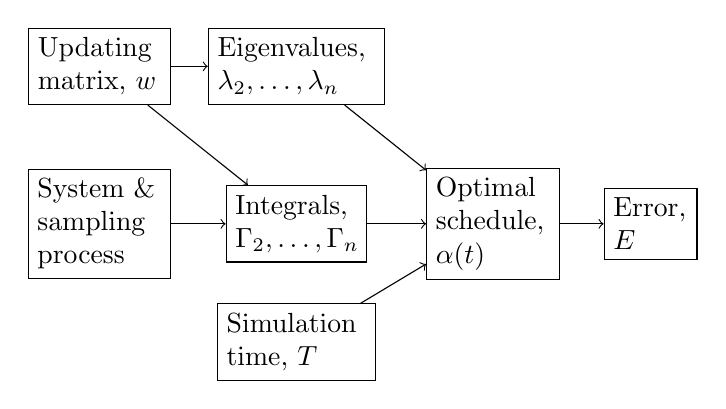
\begin{tikzpicture}
  \node[draw, text width={width("Updating ")}]
    (w) at (0, 3) {Updating \\matrix, $w$};

  \node[draw, text width={width("System  11")}]
    (sys) at (0, 1) {System \& \\sampling \\process};

  \node[draw, text width={width("Eigenvalues, ")}]
    (lambda) at (2.5, 3) {Eigenvalues, \\$\lambda_2, \dots, \lambda_n$};

  \node[draw, text width={width("Integrals, ")}]
    (gamma) at (2.5, 1) {Integrals, \\$\Gamma_2, \dots, \Gamma_n$};

  \node[draw, text width={width("Simulation ")}]
    (T) at (2.5, -0.5) {Simulation \\time, $T$};

  \node[draw, text width={width("Schedule ")}]
    (alpha) at (5, 1) {Optimal schedule, \\ $\alpha(t)$};

  \node[draw, text width={width("Error ")}]
    (err) at (7, 1) {Error, \\ $\Err$};

  \draw[->] (w) edge (lambda)
            (w) edge (gamma)
            (sys) edge (gamma)
            (lambda) edge (alpha)
            (gamma) edge (alpha)
            (T) edge (alpha)
            (alpha) edge (err);

\end{tikzpicture}
\caption{
  \label{fig:vardep}
  Dependence of variables in the method of computing
  the optimal schedule.
}
\end{figure}


\subsection{\label{sec:band-matrix}
Homogeneous updating schemes}



Many commonly-used updating schemes
can be characterized by a rigid wave packet
whose center drifts with the current bin.
%
We call these schemes homogeneous,
or translationally invariant.
%
An example is the Gaussian updating scheme
used in metadynamics.
%
Homogeneous updating schemes have significantly fewer
parameters than the general case,
and the multiplication of the updating matrix,
$\mathbf w$,
can be reduced to a convolution with the wave packet,
or the updating kernel.
%
Thus,
the eigenvalues, $\lambda_k$'s, of $\mathbf w$
can be readily computed and manipulated
via the shape of the updating kernel.



While the translational invariance of
the updating scheme
naturally suits a periodic variable\cite{dama2014},
it can also be extended to a non-periodic variable
by imposing the reflective boundary condition.
%
For simplicity, we shall assume that the target
distribution is flat, or $p_i = 1/n$, below.



\subsubsection{\label{sec:bandkernel}
Updating kernel and eigenvalues}



It is natural to introduce a homogeneous updating scheme
for a periodic variable\cite{dama2014}.
%
Consider the following matrix, $\mathbf w$,
%
\begin{equation}
  w_{ij}
  =
  \mu_{i-j}
  +
  \mu_{i-j+n}
  +
  \mu_{i-j-n}
  ,
\label{eq:w_band_pbc}
\end{equation}
%
where
$\mu_{-b}, \dots, \mu_b$ ($b \le n/2$)
are a set of numbers satisfying
%
\begin{equation}
  \mu_{-b} + \cdots + \mu_b = 1
  ,
\label{eq:mu_normalization}
\end{equation}
%
and $\mu_l = 0$ for $l > b$.
%
Particularly,
we shall only consider symmetric kernels
that satisfy
%
\begin{equation}
  \mu_i = \mu_{-i}
  .
\label{eq:mu_symm}
\end{equation}
%
If $b = n/2$, then $\mu_{-b}$ is dropped
from Eq. \eqref{eq:mu_normalization}.
%
These numbers constitutes a \emph{updating kernel}.


This above matrix, $\mathbf w$,
being symmetric to the indices $i$ and $j$,
satisfies Eqs. \eqref{eq:w_sumj}-\eqref{eq:w_balance},
for the flat distribution $p_i = 1/n$.
%
To find the eigenvectors,
we note that for a periodic variable $\varphi_i$,
the out-of-boundary values are defined by
%
\begin{equation}
  \varphi_i = \varphi_{i \pm n},
\label{eq:phi_pbc}
\end{equation}
%
such that $i \pm n$ lies in between $1$ and $n$.
%
We then have
%
\begin{equation}
  \sum_{ j = 1 }^n
    w_{ij} \, \varphi_j
  =
  \sum_{ j = 1 - n }^{ 2 \, n }
    \mu_{i - j} \, \varphi_j
  =
  \sum_{ l = -b }^{ b }
    \mu_l \, \varphi_{ i - l}
  .
\label{eq:wmul_to_convol}
\end{equation}
%
\note{The derivation of the first step of
  Eq. \eqref{eq:wmul_to_convol}:
$$
\begin{aligned}
  \sum_{j = 1}^n
    w_{ij} \, \varphi_j
  &=
  \sum_{j = 1}^n
    \mu_{i - j} \, \varphi_j
  +
  \sum_{j = 1}^n
    \mu_{i - j - n} \, \varphi_j
  +
  \sum_{j = 1}^n
    \mu_{i - j + n} \, \varphi_j
  \\
  &=
  \sum_{j = 1}^n
    \mu_{i - j} \, \varphi_j
  +
  \sum_{j = 1+n}^{2 \, n}
    \mu_{i - l} \, \varphi_l
  +
  \sum_{j = 1-n}^0
    \mu_{i - j + n} \, \varphi_j
  \\
  &=
  \sum_{j = 1-n}^{2 \, n}
    \mu_{i - j} \, \varphi_j
  .
\end{aligned}
$$
The second step of Eq. \eqref{eq:wmul_to_convol}
follows from the constraint $\mu_l = 0$ for $|l| > b$.

Similarly,
for the left eigenvector, we have
$$
  \sum_{ i = 1 }^n
    \varphi_i \, w_{ij}
  =
  \sum_{ l = -b }^b
    \varphi_{j - l} \, \mu_{-l}
  .
$$
But due to the symmetry Eq. \eqref{eq:mu_symm},
it is identical to \eqref{eq:wmul_to_convol}.
}

Thus,
we may construct a set of orthonormal eigenvectors,
$\pmb\varphi^{(1)}, \dots, \pmb\varphi^{(n)}$,
as
\begin{equation}
  \phi^{(k)}_j
  =
  \phi_{kj}
  =
  \frac{1}{\sqrt n}
  \exp
  \left[
    \ii
    \frac{ (k - 1) \, j \, 2 \, \pi }
         {            n             }
  \right]
  ,
  \notag
\end{equation}
%
with the eigenvalues being
%
\begin{equation}
  \lambda_k
  =
  \mu_0
  +
  2 \,
  \sum_{ l = 1 }^b
  \mu_l
  \cos
  \frac{ (k - 1) \, l \, 2 \, \pi }
       {            n             }
  .
  \label{eq:wband_eigenvalue_pbc}
\end{equation}
%
\note{Consider the unnormalized version
  $$
  \Phi^{(k)}_j =
  \exp\left[
    \frac{ ( k - 1 ) \, j \, 2 \, \pi }
         {              n             }
    \ii
  \right]
  ,
  $$
  we have
  $$
  \begin{aligned}
  \sum_{j = 1}^n
    w_{ij} \, \Phi^{(k)}_j
  &=
  \sum_{l = -b}^b
    \mu_l \, \Phi^{(k)}_{i - l}
  \\
  &=
  \mu_0 \, \Phi^{(k)}_i
  +
  \sum_{l = 1}^b
    \mu_l \,
    \left[ \Phi^{(k)}_{i - l} + \Phi^{(k)}_{i + l} \right]
  \\
  &=
  \Phi^{(k)}_i \,
  \left[
    \mu_0
    +
    2 \sum_{l = 1}^b
      \mu_l \, \cos
      \frac{ (k - 1) \, l \, 2 \, \pi }
           {            n             }
  \right]
  .
  \end{aligned}
  $$
  The term in the square brackets is the eigenvalue given by
  Eq. \eqref{eq:wband_eigenvalue_pbc}.
}
%
Note, however, the two-fold degeneracy as
$\lambda_{n - k + 2} = \lambda_k$.



We now adapt the above formulae to a non-periodic variable.
%
We shall use the reflective boundary condition\cite{bussi2006},
and modifies the form of the updating matrix, $\mathbf w$, as
%
%
\begin{equation}
  w_{ij}
  =
  \mu_{ i - j }
  +
  \mu_{ i + j - 1 }
  +
  \mu_{ i + j - 2 n - 1 },
  \label{eq:w_band}
\end{equation}
%
Again the updating kernel satisfies
Eqs. \eqref{eq:mu_normalization}
and
\eqref{eq:mu_symm}.
%
However,
the radius $b$ only need to be less than $n$
instead of $n/2$.
%
The last two terms
on the right-hand side of \eqref{eq:w_band} are added
to avoid unintended distortion\cite{dickson2011, mcgovern2013}
to the equilibrium distribution $p_i = 1/n$\cite{bussi2006},
such that Eqs. \eqref{eq:w_sumj}-\eqref{eq:w_balance}
are satisfied.

To compute the eigenvectors,
we shall replace Eq. \eqref{eq:phi_pbc}
and redefine the out-of-boundary values
of $\varphi_j$ as
%
\begin{equation}
  \varphi_j
  =
  \begin{dcases}
    \varphi_{ 1 - j }           & \mathrm{for \;} j \le 0, \\
    \varphi_{ 2 \, n + 1 - j }  & \mathrm{for \;} j > n,
  \end{dcases}
\label{eq:phi_refl}
\end{equation}
%
One can show that Eq. \eqref{eq:wmul_to_convol}
still holds.
%
\note{The derivation of Eq. \eqref{eq:wmul_to_convol}
  in this case is similar,
  $$
  \begin{aligned}
    \sum_{j = 1}^n w_{ij} \, \varphi_j
    &=
    \sum_{j = 1}^n
      \mu_{i - j} \, \varphi_j
    +
    \sum_{j = 1}^n
      \mu_{i + j - 1} \, \varphi_j
    +
    \sum_{j = 1}^n
      \mu_{i + j - 2 \, n - 1} \, \varphi_j
    \\
    &=
    \sum_{j = 1}^n
      \mu_{i - j} \, \varphi_j
    +
    \sum_{l = 1 - n}^0
      \mu_{i - l} \, \varphi_l
    +
    \sum_{l = n + 1}^{ 2 \, n }
      \mu_{i - l} \, \varphi_l
    \\
    &=
    \sum_{j = 1 - n}^{ 2 \, n}
      \mu_{i - j} \, \varphi_j.
  \end{aligned}
  $$
}
%
Thus, it is also possible to construct
$n$ orthonormal eigenvectors,
$\pmb\varphi^{(1)}, \dots, \pmb\varphi^{(n)}$,
as
%
\begin{equation}
\varphi^{(k)}_i
=
\varphi_{k i}
=
\sqrt{
    \frac{ 2 - \delta_{k, 1} }
         {       n           }
     }
   \cos \frac{ ( k - 1) \, \left( i - \frac 1 2 \right) \, \pi}
            {                  n                         }.
\notag
%\label{eq:wband_eigenvector_refl}
\end{equation}
%
with eigenvalues
%
\begin{align}
  \lambda_k
  &=
  \mu_0
  +
  2
  \sum_{l = 1}^b
    \mu_l
    \cos \frac{(k - 1)  \, l \pi}{n}
  \label{eq:wband_eigenvalue_refl}
\end{align}
%
\note{We derive the above two equations below.

  To simplify the calculation,
  let us first consider the unnormalized eigenvectors,
  $$
  \Phi^{(k)}_i
  =
  \cos \frac{ \left( i - \frac 1 2 \right) (k - 1) \, \pi}{n},
  $$
  which satisfies the reflective boundary condition,
  Eq. \eqref{eq:phi_refl}.
  %
  So
  $$
  \begin{aligned}
  \sum_{i = 1}^n
    \Phi^{(k)}_i \, w_{ij}
  &=
  \sum_{l = -b}^b
    \Phi^{(k)}_{j - l} \, \mu_l
  \\
  &=
    \Phi^{(k)}_j \, \mu_0
  + \sum_{l=0}^{b}
    \mu_l \,
    \left[
      \Phi^{(k)}_{j-l}
      +
      \Phi^{(k)}_{j+l}
    \right]
  \\
  &= \Phi^{(k)}_j \, \lambda_k,
  \end{aligned}
  $$
  with $\lambda_k$ given by Eq. \eqref{eq:wband_eigenvalue_refl}.

  \hrulefill

  Next, let us compute the normalization factor.
  %
  If $k = 1$, $\Phi^{(1)}_i = 1$, and
  $
  \sum_{i = 1}^n \left( \Phi^{(1)}_i \right)^2 = n.
  $
  For $k \ge 2$,
  $$
  \begin{aligned}
    \sum_{i = 1}^n \cos^2 \left[\left(i - \frac1 2 \right) a\right]
    &=
    \frac n 2
    +
    \frac 1 2
    \sum_{i = 1}^n \cos\left[(2 i - 1)\, a \right]
    =
    \frac n 2,
  \end{aligned}
  $$
  where $a = \frac{k-1}{n} \pi$.
  Thus, the normalization factor $\sqrt{(2 - \delta_{k1})/n}$
  encompasses both cases.

  \hrulefill

  To show the column-wise orthogonality,
  we need a lemma, for $a = q \, \pi/n$,
  with $q$ a positive integer.
  $$
  \begin{aligned}
  \sum_{k = 1}^n \cos[(k - 1) \, a]
  &=
  1 + \cos a + \dots + \cos[(n - 1) \, a]
  \\
  &=
  \frac{
        \sin\frac a 2
      + \sin \left[ \left( n - \frac 1 2 \right) a \right]
      }
      {
        2 \, \sin \frac a 2
      }
  \\
  &=
  \frac{ 1 - (-1)^q } { 2 }
  = \operatorname{odd}(q),
  \end{aligned}
  $$
  %
  where, we have used
  $\sin \left[ \left( n - \frac 1 2 \right) a \right]
  = \sin \left( q \, \pi - \frac a 2 \right)
  = -(-)^q\sin\frac a 2.$
  %
  and $\operatorname{odd}(q)$
  yields $1$ for odd $q$ or $0$ otherwise.
  %
  Adding the case of $q = 0$, where the sum yields $n$,
  we get
  $$
  \sum_{k = 1}^n
    \cos\left[(k - 1) \, \frac { q \, \pi } { n }  \right]
  = n \, \delta_{q, 0}
  + \operatorname{odd}(q).
  $$

  Now, for the orthogonality,
  $$
  \begin{aligned}
    \sum_{k = 1}^n
    \Phi^{(k)}_i \, \Phi^{(k)}_j
    &=
    \frac 1 2
    \sum_{k = 1}^n
    \left[
      \cos \tfrac{ (i - j) (k - 1) \, \pi }
                 {         n              }
      +
      \cos \tfrac{ (i + j - 1) (k - 1) \, \pi }
                 {             n              }
    \right]
    \\
    &=
    \frac 1 2
    \left[
      n \, \delta_{i, j}
      +
      \operatorname{odd}(i - j)
      +
      \operatorname{odd}(i + j - 1)
    \right]
    \\
    &=
    \frac n 2 \, \delta_{i, j}
    + \frac 1 2.
  \end{aligned}
  $$
  where we have used the fact
  that $i - j$ shares the parity with $i + j$
  in the last step.
  %
  So
  $$
    \sum_{k = 1}^n
    \varphi^{(k)}_i \, \varphi^{(k)}_j
    =
    \frac 2 n
    \sum_{k = 1}^n
    \Phi^{(k)}_i \, \Phi^{(k)}_j
    -
    \frac 1 n
    =
    \delta_{i, j}.
  $$
}
%


Note that Eq. \eqref{eq:wband_eigenvalue_refl}
differs from Eq. \eqref{eq:wband_eigenvalue_pbc}
by a factor of $2$
in the argument of the cosine function.
%
We may unify the two as
%
\begin{equation}
  \lambda_k
  =
  \mu_0
  +
  2
  \sum_{ l = 1 }^b
    \mu_l \,
    \cos \frac{ (k - 1) \, l \, g \, \pi }
              {            n             }
  ,
  \label{eq:wband_eigenvalue}
\end{equation}
%
where the degeneracy $g$ is $2$
for the periodic case,
or $1$ otherwise.
%
Equation \eqref{eq:wband_eigenvalue}
shows that the eigenvalues, $\lambda_k$,
of the updating scheme
is the cosine transform of
the updating kernel.
%
So, for the updating scheme to be stable,
the cosine transform of the kernel
must be nonnegative.
%
If this is not so,
we can modify the kernel
using the technique described
in Sec. \ref{sec:stabilize_wband}.

We discuss two special cases below.



\subsubsection{\label{sec:nnscheme}
Nearest-neighbor updating scheme}



If $\mu_2 = \dots = \mu_b = 0$,
the matrix $\mathbf w$ is tridiagonal,
%%
%\begin{equation}
%\arraycolsep=3.6pt\def\arraystretch{1.4}
%\mathbf w
%=
%\left(
%  \begin{array}{cccccccc}
%    1 - \mu_1   & \mu_1 & 0 & \dots & 0 \\
%    \mu_1 & 1 - 2 \, \mu_1  & \mu_1 & \dots & 0 \\
%    \vdots & &  & & \vdots \\
%    0 & \dots & \mu_1 & 1 - 2 \, \mu_1  & \mu_1 \\
%    0 & \dots & 0 & \mu_1 & 1 - \mu_1
%  \end{array}
%\right).
%\label{eq:wnn}
%\end{equation}
%%
%We have
and the eigenvalues are
\begin{equation}
  \lambda_k
  =
  1 -
  4 \, \mu_1 \sin^2
  \frac{ (k - 1) \, g \, \pi }
       {       2 \, n        }
  .
\label{eq:wnn_eigenvalue}
\end{equation}
%
Thus, for this updating matrix to be stable,
we need
$\min \lambda_k = \lambda_n > 0$,
or
\begin{equation}
  \mu_1 <
  \begin{dcases}
    \frac 1 4
    & \mathrm{periodic, \;} n \mathrm{ \; even,}
    \\
    \frac 1 4
    \cos^{-2}\frac{  \pi   }
                  { 2 \, n }
    & \mathrm{otherwise}.
  \end{dcases}
\label{eq:nn_stable}
\end{equation}






\subsubsection{Gaussian updating scheme}



The Gaussian updating kernel is commonly
adopted by metadynamics simulations.
%
Below we show that the corresponding updating scheme
is stable, albeit less effective
in reducing short-wavelength noises.



We start by defining
a continuous limit
for $b = n - 1 \gg 1$:
$x = l \, \Delta x$,
and
$\mu_l = \mu(x) \, \Delta x$,
where
$\Delta x = \pi/n$
is the bin size.
%
Then
Eq. \eqref{eq:wband_eigenvalue}
can be approximated by an integral:
%
\begin{equation}
\lambda_k
=
2 \int_0^\pi
  \mu(x) \, \cos \bigl[ (k-1) \, x \bigr] \, dx,
\label{eq:lambda_int}
\end{equation}
%
with the normalization
%
\begin{equation}
1 = 2 \int_0^\pi \mu(x) \, dx.
\label{eq:mx_normalization}
\end{equation}



Particularly,
for the Gaussian updating kernel,
if $\Delta x \ll \sigma \ll 1$,
we can extended
the upper limit of the integrals
in Eqs. \eqref{eq:lambda_int}
and \eqref{eq:mx_normalization}
to infinity, and
%
\begin{equation}
\mu(x)
=
\frac{            1            }
     { \sqrt{ 2 \pi \sigma^2 } }
%
\exp\left(
      -\frac{       x^2     }
            { 2 \, \sigma^2 }
    \right),
\notag
\end{equation}
%
%
The eigenvalues are given by
%
\begin{align}
\lambda_k
&=
\exp\left[
      -\frac{ (k - 1)^2 \, \sigma^2 }
            {           2           }
    \right]
\notag
\\
&=
\exp\left[
      -\frac{ \pi^2 }{ 2 }
      \left(
        \frac{ k - 1 }
             {   n   }
      \right)^2
      \left(
        \frac{  \sigma }
             { \Delta x }
      \right)^2
    \right]
.
\notag
%\label{eq:lambda_Gaussian}
\end{align}
%
The eigenvalues are all positive,
suggesting stability of the updating scheme.


%However,
%as $\sigma/\Delta x \gg 1$,
%the smallest eigenvalue
%%
%$$
%\lambda_n
%\approx
%\exp\left(
%      -\frac{ n^2 \, \sigma^2 }
%            {        2        }
%    \right)
%=
%\exp\left[
%      -\frac{ \pi^2 }{ 2 }
%      \left(
%        \frac{  \sigma }
%             { \Delta x }
%      \right)^2
%    \right]
%.
%$$
%%
%is exponentially small.
%%
%This means that
%the optimal value of $\lambda$
%given by Eq. \eqref{eq:optimal_lambda_approx}
%would be too small in practice,
%for it requires $\lambda < 2 \, \lambda_n$.
%%
%In other words,
%with a reasonable $\lambda$,
%the error of the last few fluctuation modes
%will always decay suboptimally,
%accordingly to Eq. \eqref{eq:error_asym_invt}.
%%
%However, since these modes
%represent short wavelength fluctuations,
%and these modes may be in
%the system under consideration.
%%
%Thus,
%we can truncate the sum of the error function
%in Eq. \eqref{eq:error_asym_invt}
%at some $k_{\max}$,
%which corresponds to a minimal length scale
%$l_{\min} = \Delta x \, (n /k_{\max}) = \pi/k_{\max}$
%greater than $\sigma$.
%%
%Then,
%$$
%\lambda_{ k_{\max} }
%\approx
%\exp\left(
%      -\frac{ k_{\max}^2 \, \sigma^2 }
%            {           2            }
%    \right)
%=
%\exp\left(
%      -\frac{  \pi^2 \, \sigma^2    }
%            {    2 \, l_{\min}^2  }
%    \right).
%$$



\subsubsection{\label{sec:stabilize_wband}
Stabilization}



A practical problem of using homogeneous updating scheme
is the following.
%
A homogeneous updating scheme
specified by an arbitrary set of numbers
$\mu_1, \dots, \mu_b$, ($b < n - 1$),
is not necessarily stable
with all nonnegative eigenvalues.
%
%
For example, the nearest-neighbor updating scheme
is unstable if Eq. \eqref{eq:nn_stable} is violated.
%
Even the Gaussian updating scheme can be unstable
if the updating kernel is truncated.
%
Below we show how to minimally modify
the updating kernel
to meet the stability criteria.
%
\note{The relative code is \texttt{trimwindow()} in \texttt{invt.h}.
}


The key is the observation of Eq. \eqref{eq:wband_eigenvalue}
that the eigenvalues are related to the updating kernel
by a cosine transform,
and thus the relationship can be readily inverted.
%
For the periodic case,
the inversion formula is
%
\begin{equation}
  \mu_l
  =
  \frac 1 n
  \sum_{ k = 1 }^n
  \lambda_k
  \cos \frac{ (k - 1) \, l \, 2 \, \pi }
            {            n             }
  .
\label{eq:mu_from_lambda_pbc}
\end{equation}


For a non-periodic variable,
the explicit inversion formula is
%
\begin{align}
  \mu_l
  =
  \frac 1 { 2 \, n }
  \sum_{ k = 1 }^{ 2 \, n }
    \lambda_{ k } \,
    \cos \frac{ (k - 1) \, l \, \pi }
              {            n        }
  ,
\label{eq:mu_from_lambda_refl}
\end{align}
%
where
we have defined
$\lambda_k \equiv \lambda_{n + 2 - k}$
for $k = n + 2, \dots, 2 \, n$,
as well as
%
\begin{align}
  \lambda_{ n + 1 }
  =
  (-1)^{ n - 1 }
  \left[
    \lambda_1
    +
    2 \, \sum_{ k = 2 }^{ n }
      (-1)^{k - 1} \, \lambda_k
  \right]
  ,
\label{eq:lambdan}
\end{align}
to satisfy the constraint $\mu_n = 0$.
%
\note{Eq. \eqref{eq:lambdan}
ensures that the $\mu_n$
computed from Eq. \eqref{eq:mu_from_lambda_refl}
vanishes.

The inversion formula is derived from the cosine transform.
  %
  If we define $\mu_n = 0$ and
  %
  \begin{align}
    \mu_{ 2 n - l } = \mu_l
    \quad
    \mathrm{for\;} l = 1, \dots, n - 1,
  \notag
  %\label{eq:mu_reflection}
  \end{align}
  %
  then Eq. \eqref{eq:wband_eigenvalue_refl} can be rewritten as
  %
  \begin{align}
    \lambda_{k+1}
    =
    \sum_{ l = 0 }^{ 2 \, n - 1 }
    \mu_l \, \cos \frac{ k \, l \, \pi } { n }.
  \notag
  %\label{eq:lambda_cosine_sum}
  \end{align}
  %
  This formula for $\lambda_{k+1}$
  can be readily extended to $k = 2 \, n - 1$,
  and we have
  %
  \begin{align}
    \lambda_{ 2 \, n + 1 - k } = \lambda_k.
    \label{eq:lambda_reflection}
  \end{align}
  %
  Thus,
  %
  $$
  \begin{aligned}
    \sum_{ k = 0 }^{ 2 \, n - 1 }
      \lambda_{ k + 1 } \,
      \cos \frac{ k \, p \, \pi }
                {      n        }
    &=
    \sum_{ k = 0 }^{ 2 \, n - 1 }
      \sum_{ l = 0 }^{ 2 \, n - 1 }
        \mu_l \,
        \cos \frac{ k \, l \, \pi }
                  {      n        }
        \cos \frac{ k \, p \, \pi }
                  {      n        }
    \\
    &=
    \sum_{ l = 0 }^{ 2 \, n - 1 }
      \frac{ \mu_l } { 2 }
      \sum_{ k = 0 }^{ 2 \, n - 1 }
        \cos \frac{ k \, (p + l) \, \pi }
                  {      n        }
                  +
        \cos \frac{ k \, (p - l) \, \pi }
                  {      n        }
    \\
    &=
    \sum_{ l = 0 }^{ 2 \, n - 1 }
      \mu_l \, n \left(
        \delta_{ p + l - 2 \, n, 0 }
        +
        \delta_{ p - l, 0 }
      \right)
    \\
    &=
    n \, \left( \mu_p + \mu_{ 2 \, n - p} \right)
    =
    2 \, n \, \mu_p.
  \end{aligned}
  $$
  This entails
  $$
  \begin{aligned}
    \mu_l
    &=
    \frac{    1   }
         { 2 \, n }
    \sum_{ k = 0 }^{ 2 \, n - 1 }
      \lambda_{ k + 1 } \,
      \cos \frac{ k \, l \, \pi }
                {      n        }
              \\
    &=
    \frac{    1   }
         { 2 \, n }
    \left[
      \lambda_1
      +
      (-1)^l \, \lambda_{n + 1}
      +
      2 \sum_{ k = 1 }^{ n - 1 }
        \lambda_{ k + 1 } \,
        \cos \frac{ k \, l \, \pi }
                  {      n        }
    \right],
  \end{aligned}
  $$
  where we have used Eq. \eqref{eq:lambda_reflection}
  in the last step.

  However, we are usually given only $\lambda_1, \dots, \lambda_n$
  without $\lambda_{n + 1}$.
  %
  Fortunately, we can deduce the latter from
  the condition that $\mu_n = 0$, which means
  $$
  \begin{aligned}
    0 = \mu_n
    =
    \frac{1}{n}
    \left[
      \frac{ \lambda_1 + (-1)^n \, \lambda_{n+1} }
           {               2                     }
      +
      \sum_{ k = 1 }^{ n - 1 }
      \lambda_{k+1} (-1)^k
    \right].
  \end{aligned}
  $$
  This allows us to solve for $\lambda_{ n + 1 }$,
  yielding Eq. \eqref{eq:lambdan}


  Some examples for checking.
  For $n = 2$,
  $\lambda_3
  = \mu_0 - 2 \, \mu_1
  = -(\lambda_1 - 2 \, \lambda_2)$,
  and
  $$
  \begin{aligned}
  \mu_0
  &=
  \lambda_2,
  \\
  \mu_1
  &=
  \frac{ \lambda_1 - \lambda_2 }
       {           2           }
  .
  \end{aligned}
  $$
  For $n = 3$,
  $\lambda_4
  = \mu_0 - 2 \, \mu_1 + 2 \, \mu_2
  = \lambda_1 - 2 \, \lambda_2 + 2 \, \lambda_3$,
  and
  $$
  \begin{aligned}
  \mu_0
  &=
  \frac{ 1 } { 3 }
  \left(
    \lambda_1 + 2 \, \lambda_3
  \right)
  ,
  \\
  \mu_1
  &=
  \frac{ 1 } { 3 }
  \left(
    \frac 3 2 \lambda_2
    -
    \frac 3 2 \lambda_3
  \right)
  ,
  \\
  \mu_2
  &=
  \frac{ 1 } { 3 }
  \left(
    \lambda_1
    -
    \frac 3 2 \lambda_2
    +
    \frac 1 2 \lambda_3
  \right)
  .
  \end{aligned}
  $$
}

Now given a updating kernel, $\mu_1, \dots, \mu_n$,
we can compute the eigenvalues from
Eq. \eqref{eq:wband_eigenvalue}.
%
By replacing negative eigenvalues with zeros and
using Eq. \eqref{eq:mu_from_lambda_pbc}
or \eqref{eq:mu_from_lambda_refl},
we get a new updating kernel
$\mu^\mathrm{new}_1, \dots, \mu^\mathrm{new}_{n - 1}$,
which is stable by construction.
%
However, the new kernel
is widened
as it contains $n/g - 1$ instead of $b$ entries.
If we truncate the new updating kernel
at a radius of $b$ bins,
the stability problem remains
albeit, hopefully, becomes less severe
(in terms of the most negative eigenvalue).
%
Thus, to obtain a stable updating kernel
without increasing the radius $b$,
we have to iterate the above process many times.
The resulting algorithm is the following.


%
\begin{enumerate}
  \item
    Given a updating kernel $\mu_1, \dots, \mu_b$,
    compute the eigenvalues
    $\lambda_0, \dots, \lambda_{n-1}$
	from Eq. \eqref{eq:wband_eigenvalue}.
  \item
    If all eigenvalues are nonnegative,
    we are done, and exit the loop.
  \item
    Otherwise, replace negative eigenvalues by zeros,
    and compute a new updating kernel,
    $\mu_1, \dots, \mu_b$ from
    Eq. \eqref{eq:mu_from_lambda_pbc}
    or
    \eqref{eq:mu_from_lambda_refl}.
    Set $\mu_l = 0$ for $l > b$.
    Go to step 1.
\end{enumerate}



\subsection{\label{sec:cmpschemes}
Comparison of updating schemes}


Now that we can compute the optimal schedule
for a given updating scheme,
can we also compare different updating schemes
and pick the best one?
%
Below we address this question
in the asymptotic, or long simulation time,
limit.


\subsubsection{\label{sec:optWL}
Asymptotic optimality of the single-bin (WL) scheme}



We shall first show,
directly from Eq. \eqref{eq:error_asym1},
that the single-bin scheme is asymptotically optimal.
%
Consider a class of $\mathbf w$ matrices
sharing the same set of eigenvectors,
hence same $\Gamma_k$'s,
but with different positive eigenvalues,
$\lambda_k$'s.
%
Using the Cauchy-Schwarz inequality, we have,
for any set of nonnegative numbers, $c_k$'s,
%
\begin{align}
&
\left(
  \int_0^T dt
    \sum_{k = 2}^n
      \Gamma_k \, \dot u_k^2\bigl( q(t) \bigr)
\right)
%
\left(
  \int_0^T dt
    \sum_{k = 2}^n
      \Gamma_k \, c_k^2
\right)
%
\notag
\\
&
\qquad \qquad
\ge
\left(
  \int_0^T dt
    \sum_{k = 2}^n
      \Gamma_k \, c_k \, \dot u_k \, \bigl( q(t) \bigr)
\right)^2
\notag
\\
&
\qquad \qquad
=
\left(
  \sum_{k = 2}^n \Gamma_k \, c_k
    \left[
      1 - e^{ -\lambda_k \, q(T) }
    \right]
\right)^2.
\label{eq:CSineq}
\end{align}
%
This inequality follows from the non-negativity of
the following quadratic polynomial of $Y$,
$$
\int_0^T
  dt \sum_{k = 2}^n \Gamma_k \,
    \left( \dot u_k \, Y - c_k \right)^2
  \equiv
  A \, Y^2 + B \, Y + C
%\ge 0,
$$
which implies a non-positive discriminant,
$B^2 - 4 \, A \, C$.
%
Note that the last expression of \eqref{eq:CSineq}
depends on the curve, $q(t)$ ($0 < t < T$),
only through the endpoint value, $q(T)$,
which is fixed in the variation process.
%
Thus, the inequality sets a lower bound
of the error $\Err$
given in Eq. \eqref{eq:error_asym1}.
%
The equality is achieved
if $\dot u_k\left( q(t) \right) = c_k$
for all $k = 2, \dots, n$ at any $t$,
up to a multiplicative factor.
%
Solving this set of equations yields
%
\begin{equation}
  \alpha(t) = \frac{              1             }
                   { \lambda_k \, (t + t_{k0} ) },
\label{eq:alpha_invtk}
\end{equation}
with
\begin{equation}
  t_{k0} = \frac{             T            }
                { e^{ \lambda_k q(T) } - 1 }.
\label{eq:tk0}
\end{equation}
%
Such a solution is possible only if
%
\begin{equation}
\lambda_2 = \dots = \lambda_n.
\end{equation}
%
In this case,
all $t_{k0}$'s also share the same value,
$t_0$ by Eq. \eqref{eq:tk0},
such that
$u_k = (t + t_0) / (T + t_0)$,
and
$c_k \propto 1/(T + t_0)$
for $k \ge 2$.
%
The asymptotic error is then
\begin{align}
  E_A
  =
  \frac{       T     }
       { (T + t_0)^2 }
  \sum_{ k = 2 }^n
    \Gamma_k
  .
\label{eq:error_singlebin}
\end{align}
%
If we further assume that $\lambda_2 = 1$,
the optimal schedule given by Eq. \eqref{eq:alpha_invtk}
recovers Eq. \eqref{eq:alpha_invt1}.
%
\note{We add some steps for the above solution.
  Integrating $\dot u_k = c_k$ yields
  \begin{equation}
  u_k(t) = c_k \left(t + t_{k0} \right).
  \label{eq:ui_solution}
  \end{equation}
  Given that $u_k(T) = 1$ and $u_k(0) = e^{-\lambda_k \, q(T)}$,
  we have
  $$
  c_k = \frac{ 1 }{ T + t_{k0} },
  \quad
  \mathrm{and\;}
  \frac{ t_{k0} } { T + t_{k0} }
  =
  e^{ -\lambda_k \, q(T) }.
  $$
  Taking the logarithm of Eq. \eqref{eq:ui_solution} yields
  $$
  -\lambda_k \, q(T) + \lambda_k \, q(t)
  = \log c_k + \log\left( t + t_{k0} \right).
  $$
  Differentiating this with respect to $t$ yields
  $$
  \lambda_k \, \alpha(t)
  =
  \frac {     1      }
        { t + t_{k0} }.
  $$
}

Since $\lambda_1$ corresponds to the mode
of a uniform shift of all $v_k$,
we can freely set $\lambda_1$ to $\lambda_2$
without changing the nature of the updating scheme.
%
Now an updating matrix $\mathbf w$
with identical eigenvalues
is essentially a multiple of the identity matrix.
%
Thus, if no eigenvalue $\lambda_k$ is zero,
then in terms of asymptotic convergence,
the single-bin scheme adopted in the WL algorithm
is most efficient.
%

Note that
since we only optimized the asymptotic error,
the inverse-time schedule is optimal
only in the long time limit,
but not necessarily so for a finite-length simulation.
%
For example, consider a system that is initially
prepared under a fixed $\alpha_0$
at the beginning of the schedule $\alpha(t)$.
%
Then for shorter times, $T \approx 0$,
the error, dominated by the residual error
given by Eq. \eqref{eq:error_res1},
is clearly smaller if some eigenvalues
are less than $1.0$ (the single-bin case).
%
%In practice, real simulations
%may have long achieved the desired precision
%before reaching the asymptotic regime,
%especially if the updating matrix
%has some $\lambda_k$'s close to $0$.


\subsubsection{\label{sec:optscheme}
Cardinal updating schemes}


We can also generalize
the single-bin scheme to a class of
optimal updating schemes
that allow zero eigenvalues.
%
For example,
if we can assume that the PMF is sufficiently smooth
such that the error modes can be limited to $k \le K$.
%
Then we can construct an updating scheme with
$$
\lambda_1 = \cdots = \lambda_K = 1,
\mathrm{\; and \;}
\lambda_{K+1} = \cdots = \lambda_n = 0.
$$
%
Then,
Eq. \eqref{eq:error_singlebin} is modified to
$$
  E
  =
  \frac {       T     }
        { (T + t_0)^2 }
  \sum_{ k = 2 }^K
    \Gamma_k.
$$
The optimal schedule of these schemes
remains to be the inverse-time schedule,
given by Eq. \eqref{eq:alpha_invt1}.
%
Below, we construct these schemes for
the homogeneous case.

For a periodic variable, if we demand
%
$$
\begin{aligned}
&
\lambda_1 = \cdots = \lambda_{K+1}
= \lambda_{n-K+1} = \cdots = \lambda_n = 1,
\\
&
\lambda_{K+2} = \cdots = \lambda_{n-K} = 0,
\end{aligned}
$$
for $K \ge 1$, then by using
Eq. \eqref{eq:mu_from_lambda_pbc},
we get
\begin{equation}
  \mu_l
  =
  \frac{
    \sin
    \dfrac{ (2 K + 1) \, l \, \pi }
         {              n        }
  }
  {
    n \, \sin \dfrac{ l \, \pi } { n }
  }
  .
  \label{eq:mu_cardinal_pbc}
\end{equation}
\note{Derivation.
$$
\begin{aligned}
\mu_l
&=
\frac 1 n \sum_{k = 0}^{n-1} \lambda_{k+1} \cos \frac{ k \, l \, 2 \, \pi } { n }
\\
&=
\frac{1}{n}
\left(
  1 +
  \sum_{k=1}^K
  \cos \frac { k \, l \, 2 \, \pi } { n }
  +
  \sum_{k=n-K}^{n-1}
  \cos \frac { k \, l \, 2 \, \pi } { n }
\right)
\\
&=
\frac 1 n
\sum_{k=-K}^K
\cos \frac { k \, l \, 2 \, \pi } { n }
=
  \frac{
    \sin
    \dfrac{ (2 K + 1) \, l \, \pi }
         {              n        }
  }
  {
    n \, \sin \dfrac{ l \, \pi } { n }
  }
.
\end{aligned}
$$
}

For a non-periodic variable, we demand
$$
\lambda_1 = \cdots = \lambda_{K+1} = 1,
\qquad
\lambda_{K+2} = \cdots = \lambda_n = 0.
$$
Then Eq. \eqref{eq:lambdan} gives
$\lambda_n = (-1)^{n+K-1}$,
and from Eq. \eqref{eq:mu_from_lambda_refl},
we have
\begin{equation}
  \mu_l
  =
  \frac{1}{2 \, n}
  \left[
    (-1)^{n+K+l-1}
    +
    \frac{
      \sin
      \dfrac{ (2 K + 1) \, l \, \pi }
           {         2 \, n        }
    }
    {
      n \, \sin \dfrac{ l \, \pi } { 2 \, n }
    }
  \right]
  .
\end{equation}
\note{Derivation.
$$
\begin{aligned}
  \lambda_{n+1}
  &=
  (-1)^{n-1}
  \left[
    \lambda_1
    + 2 (-\lambda_2 + \lambda_3 - \cdots + (-1)^K \lambda_{K+1})
  \right]
  \\
  &=
  \begin{dcases}
    (-1)^{n-1} & K \mathrm{\; even,} \\
    (-1)^n     & K \mathrm{\; odd.}
  \end{dcases}
\end{aligned}
$$
So
$$
\begin{aligned}
  \lambda_l
  &=
  \frac{1}{2\,n}
  \left[
    1 +
    2 \sum_{k=2}^{K+1}
    \cos \frac { (k - 1) \, l \pi } { n }
    +
    (-1)^{n+K-1} (-1)^l
  \right]
  \\
  &=
  \frac{1}{2\,n}
  \left[
    (-1)^{n+K+l-1}
    +
    \sum_{k=-K}^{K}
    \cos \frac { k \, l \pi } { n }
  \right]
  .
\end{aligned}
$$

\hrulefill

Example 1. If $n = 3, K = 1$,
then $\lambda_1 = \lambda_2 = 1$, $\lambda_3 = 0$,
and $\lambda_4 = \lambda_1 - 2 \, \lambda_2 + 2 \, \lambda_3 = -1$.
%
We can verify that $\mu_0 = 1/3, \mu_1 = 1/2, \mu_2 = -1/6$.
%
Although $\mu_1 > \mu_0$, the system will not be trapped
in the current bin because of the reflective boundary condition.
%
Upon a visit to the middle bin, $j = 2$,
$v_i$ at bin $i = 1$ or $3$ is updated by $1/2 - 1/6 = 1/3$,
same as the update on bin $2$.
Upon a visit to bin $i = 1$, the three bins are updated
by $1/2 + 1/3 = 5/6$, $1/2 - 1/6 = 1/3$, and $-1/6$,
respectively.

\hrulefill

Example 2. If $n = 3, K = 2$,
then $\lambda_1 = \lambda_2 = \lambda_3 = 1$, $\lambda_4 = 1$.
We have $\mu_0 = 1, \mu_1 = \mu_2 = 0$,
recovering the single-bin scheme.

\hrulefill

Example 3. If $n = 4, K = 1$,
then $\lambda_1 = \lambda_2 = 1, \lambda_3 = \lambda_4 = 0$,
$\lambda_5 = (-1)(\lambda_1 - 2 \, \lambda_2 + 2 \, \lambda_3 - 2 \, \lambda_4 = 1$.
The kernel is given by
$\mu_0 = 1/2, \mu_1 = \sqrt{2}/8, \mu_2 = 1/4, \mu_3 = -\sqrt{2}/8$.
}





\subsubsection{\label{sec:equilerr}
Comparison to the error of the equilibrium FDS method}


As discussed in Sec. \ref{sec:FDS},
the asymptotic limit of an adaptive FDS method
is the corresponding equilibrium FDS method
with the bias potential fixed to the exact value.
%
Such a simulation delivers the maximal efficiency.

A practical question now arises.
%
In late stages of an adaptive FDS simulation,
if we are confident that the bias potential
is sufficiently accurate,
will we be better off switching to the equilibrium FDS method
to prevent possible efficiency loss
due to the adaptive updates?
%
Below, we shall show that this is unnecessary
if the simulation uses the single-bin (WL) updating scheme
with the optimal schedule, Eq. \eqref{eq:alpha_invt1}.
%
That is, the bias potential obtained from
an optimal single-bin scheme FDS simulation
will be similar in precision to that from
the ideal equilibrium FDS simulation
in long times.
%
Thus, our demonstration below serves as an alternative proof
of the optimality of the single-bin scheme.

The error of the equilibrium FDS method
depends on the precision of the histogram.
%
The error is minimized
when $v_i$'s assume the exact values,
%
and in this case,
the error came from the second term
on the right-hand side of Eq. \eqref{eq:vcorr_equil},
%
\begin{align}
  E
  &=
  \left\langle
    \sum_{ i = 1 }^ n
      p_i \,
      \left(
        \log \frac { H_i }
                   { p_i }
      \right)^2
  \right\rangle
\notag
\\
  &\approx
  \sum_{ i = 1 }^ n
    p_i \,
    \left\langle
      \left(
        \frac { H_i }
              { p_i }
        - 1
      \right)^2
    \right\rangle,
\notag
\end{align}
where
$H_i = \frac{1}{T} \sum_{t = 1}^T h_i(t)$
with
$h_i(t)$ defined by Eq. \eqref{eq:h_def}.

To make better comparison with
the error of the single-bin case,
we shall rewrite the error as
a sum over the eigenmodes.
We define
\begin{align}
  \Theta_k
  =
  \frac{ 1 } { T }
  \sum_{ t = 1 } ^ T
    \theta_k( t )
  ,
\notag
\end{align}
%
with $\theta_k(t)$ defined by Eq. \eqref{eq:eta_def}
and $\phi_{k i}$ by Eq. \eqref{eq:eig_orthonormal_cols}.
%\begin{align}
%\theta_k( t )
%=
%\sum_{ i = 1 }^ n
%\phi_{k i} \left[
%             \frac{ h_i(t) }
%                  { p_i    }
%             - 1
%           \right],
%\end{align}
%and
%\begin{align}
%\sum_{ k = 1 }^n
%  \phi_{k i} \, \phi_{k j}
%  = p_i \, \delta_{i j}.
%\end{align}
%
Then,
%
\begin{align}
  E
  =
  \sum_{ k = 1 }^n
    \left\langle
      \Theta_k^2
    \right\rangle.
\notag
%\label{eq:error_sbin_equil}
\end{align}
%
\note{Because
%
\begin{align*}
\sum_{ k = 1 }^n
  \Theta_k^2
&=
\frac{ 1 } { T^2 }
\sum_{ t, t' = 1 }^T
  \sum_{ k = 1 }^n
    \theta_k( t ) \, \theta_k( t' )
\\
&=
\frac{ 1 } { T^2 }
\sum_{ t, t' = 1 }^T
  \sum_{ i, j = 1 }^n
    \left[
      \frac{ h_i(t) }
           { p_i    }
      - 1
    \right]
    \left[
      \frac{ h_j(t') }
           { p_j     }
      - 1
    \right]
    \sum_{ k = 1 }^n
      \phi_{k \, i} \, \phi_{k \, j}
\\
&=
\frac{ 1 } { T^2 }
\sum_{ t, t' = 1 }^T
  \sum_{ i, j = 1 }^n
    \left[
      \frac{ h_i(t) }
           { p_i    }
      - 1
    \right]
    \left[
      \frac{ h_j(t') }
           { p_j     }
      - 1
    \right]
    p_i \, \delta_{i, j}
\\
&=
\sum_{ i = 1 }^n
\frac{ 1 } { T }
\sum_{ t = 1 }^T
    \left[
      \frac{ h_i(t) }
           { p_i    }
      - 1
    \right]
\frac{ 1 } { T }
\sum_{ t' = 1 }^T
    \left[
      \frac{ h_i(t') }
           { p_i     }
      - 1
    \right]
\\
&=
\sum_{ i = 1 }^n
  p_i \,
    \left(
      \frac{ \bar h_i }
           { p_i      }
      - 1
    \right)^2
.
\end{align*}
}
The sum can start from $k = 2$, for
by Eq. \eqref{eq:eigenmode1}, we have
$$
\theta_1(t)
=
\sum_{ i = 1 }^n
  \phi_{1i} \, \frac{ h_i(t) - p_i } { p_i }
=
\sum_{ i = 1 }^n h_i(t)
-
\sum_{ i = 1 }^n p_i = 0.
$$

In the long-time limit,
\begin{align*}
\left\langle
  \Theta_k^2
\right\rangle
&=
\frac{1}{T^2}
\sum_{ t, t' = 1 }^T
\langle \theta_k(t) \, \theta_k(t') \rangle
\\
&\approx
\frac{1}{T}
\sum_{ \tau = -\infty }^{ \infty }
\langle \theta_k(t) \, \theta_k(t + \tau) \rangle
\\
&=
\frac{1}{T}
\int_{-\infty}^\infty
\kappa_n(\tau) \, d\tau
=
\frac{1}{T}
\Gamma_k.
\end{align*}
%
Thus,
\begin{equation}
  E
  =
  \frac{ 1 } { T }
  \sum_{ k = 2 }^n \Gamma_k
  .
\label{eq:error_equil}
\end{equation}

Now comparing this with the error of the single-bin scheme
with the optimal schedule,
Eq. \eqref{eq:error_singlebin},
we find that the difference is negligible
in the long time limit.

Again, if we are certain that
the intrinsic PMF is sufficiently smooth,
then we can explicitly filter some error modes,
say those for $k > K$,
in the histogram, and the sum in
Eq. \eqref{eq:error_equil}
can be truncated at $k = K$.





\section{\label{sec:results}
Numerical results}



\subsection{Test system and simulation protocol}


Our test system is
a model one-dimensional system
of $n = 100$ bins,
with a flat target distribution
$p_i = 1/n$
under the reflective boundary condition.
%
%Since in the asymptotic regime,
%the distribution converges to $p_i$
%no matter the intrinsic distribution, $p^*_i$,
%we also set the latter to be flat for convenience.
For convenience,
the intrinsic distribution, $p^*_i$,
is a set to be flat as well.
%
Our goal is to observe how the fluctuating error
of the bias potential defined in Eq. \eqref{eq:error_sum}
depends on the schedule, $\alpha(t)$,
at the end of the simulation.



Initially,
we set the bias potential to zero,
$v_i \equiv 0$,
%
and equilibrate the system under
a constant updating magnitude,
$\alpha(t) = \alpha_0$.
%
After this,
we reset the origin of the time, $t$,
and started the target schedule.
%specified by either
%Eq. \eqref{eq:q_opt}
%or
%Eq. \eqref{eq:alpha_invtlambda}.


For the Gaussian updating scheme,
the kernel is truncated at
$\min\{10 \, \sigma, n - 1\}$
and numerically stabilized
using the technique
in Sec. \ref{sec:stabilize_wband}.



Since the error depends on
the underlying sampling process,
we have devised two sampling processes,
a global one and a local one.
%
Both cases were based on
Metropolis algorithm\cite{metropolis1953, newman, frenkel,
landau_binder}:
%
in each step, a new bin index $j$ was proposed
and then accepted with probability
%
$
A(i \to j) = \min\{ 1, \exp(v_i - v_j) \}.
$
However,
in the first and global sampling process,
we choose the destination $j$
randomly out of the $n$ bins.
%
This sampling process
emulates the perfect sampling process
discussed in Sec. \ref{sec:Gamma}
in the long time limit.
%
In the second or local process,
we limit the destination $j$
to the two neighbors of $i$,
$i \pm 1$, with equal probability $1/2$,
to mimic the one-step sampling process
in Sec. \ref{sec:Gamma}.
%



\subsection{Inverse-time schedule}



We first tested the theory using
the inverse-time schedule,
%
\begin{equation}
\alpha(t) = \frac{1}{\lambda \, (t + t_0) },
\label{eq:alpha_invtlambda}
\end{equation}
%
where $\lambda$ is a parameter to be optimized.
and $t_0 = 1/(\lambda \, \alpha_0)$
to smooth the transition from equilibration.
%
This schedule is analytically simpler
than the optimal schedule,
and it is studied in Appendix \ref{sec:invt_schedule}.
%
We wish to see how the final error
depends on the parameter, $\lambda$,
and if it matches the predicted value,
given by Eq. \eqref{eq:error_invt}.


\subsubsection{Single-bin (WL) updating scheme}



For the single-bin updating scheme,
we chose $\alpha_0 = 0.0001$
and ran the simulation for $t = 10^8$ steps.
%
As shown in Fig. \ref{fig:err_singlebin},
the numerical results of the terminal error agreed well with
the analytical prediction by Eq. \eqref{eq:error_invt}.
%
For both global and local sampling processes,
the optimal $\lambda$ occurred around $1.0$,
verifying Eq. \eqref{eq:alpha_invt1}.
%
%Recall that $1/\lambda$ in Eq. \eqref{eq:alpha_invtlambda}
%represents the relative updating magnitude.
%%
%Figure \ref{fig:err_singlebin} also shows
%an asymmetry of the error curve.
%A smaller than optimal value of
%the updating magnitude, $1/\lambda$,
%tends to increase the error more rapidly
%than a larger than optimal value,
%suggesting that the over-updating
%is generally preferable to the under-updating
%when the optimal value is unknown.


We also observe
that the two error functions
differed only by a multiplicative constant,
again again agreeing with the theory.
%
With identical eigenvalues,
$\lambda_1 = \cdots = \lambda_n = 1$,
the error in Eq. \eqref{eq:error_invt}
depends on the sampling process only through
the sum $\sum_{ k = 2 }^n \Gamma_k$,
which gives rise to the above multiplicative constant.


\begin{figure}[h]
\begin{center}
  \makebox[\linewidth][c]{
    \includegraphics[angle=0, width=0.95\linewidth]{fig/errsbin.pdf}
  }
  \caption{
    \label{fig:err_singlebin}
    Error, $E$, versus the
    relative updating magnitude,
    %proportionality constant,
    $1/\lambda$,
    in Eq. \eqref{eq:alpha_invtlambda}
    for the single-bin (WL) scheme.
    %
    The results have been averaged over $1000$ independent runs.
  }
\end{center}
\end{figure}



\subsubsection{Nearest-neighbor updating scheme}


As an example of the multiple-bin schemes,
we chose the nearest-neighbor updating scheme
described in Sec. \eqref{sec:nnscheme}.
%
We again find good agreement
between simulation and analytical results.
%
A new feature is that the optimal $\lambda$
depends on the simulation length, $T$.
%
As shown in Fig. \ref{fig:err_nnbr},
the normalized error, $(T + t_0) \, \Err$,
hence the optimal value of $1/\lambda$,
depended non-trivially on the simulation length, $T$,
in the global sampling case.
%
The optimal $1/\lambda$ gradually increased
with simulation length, which is in agreement with
the discussion in Sec. \ref{sec:optlambda}.
%
For the local sampling case,
the $T$-dependence was hardly visible
because of the predominantly large $\Gamma_k$'s
of the small $k$ modes.
%
The optimal $\lambda$ remained around $1.0$,
as suggested by Eq. \eqref{eq:lambda_nn_onestep}.



%To understand this dependence,
%we observe that for shorter simulations,
%long-wavelength modes
%(with larger $\lambda_k$ and smaller $k$),
%dominate the error function in Eq. \eqref{eq:error_invt}
%because of the prefactor $\lambda_k \, \Gamma_k$,
%which is inherited from
%the equilibrium error under a fixed updating magnitude,
%Eq. \eqref{eq:error_eql}.
%%
%For longer simulations,
%short-wavelength modes
%(with smaller $\lambda_k$ and larger $k$)
%become more important,
%for $\lambda_k$ also gives the decay rate
%of the $k$th mode.
%%and errors in smaller $\lambda_k$ modes
%%are harder to damp out.
%%
%This drives the optimal $\lambda$ to shift toward
%a smaller $\lambda_k$ value
%as the simulation lengthens.
%%
%Note also that while increasing $\lambda$
%also increases the error of the long-wavelength modes,
%this rate of increase is much smaller,
%as shown in the $\nu_k > 1$ branch
%in Fig. \ref{fig:err_component}.
%%
%The shift of $\lambda$, however, is less noticeable
%under the local sampling scheme,
%because longer-wavelength modes more heavily
%weighted by much larger values of $\Gamma_k$.


\begin{figure}[h]
\begin{center}
  \makebox[\linewidth][c]{
    \includegraphics[angle=0, width=0.95\linewidth]{fig/errnnbr.pdf}
  }
  \caption{
    \label{fig:err_nnbr}
    Normalized error, $(T + t_0) \, E$,
    versus the %proportionality constant,
    relative updating magnitude,
    $1/\lambda$,
    in Eq. \eqref{eq:alpha_invtlambda}
    for the nearest-neighbor updating scheme with $\mu_1 = 0.24$.
    %
    The results have been averaged over $1000$ independent runs.
  }
\end{center}
\end{figure}





%\subsection{Gaussian (metadynamics) updating scheme}
%
%
%The error of Gaussian updating scheme is similar to
%that of the nearest neighbor scheme,
%as shown in Fig \ref{fig:err_sig5}.
%%
%The dependency of the simulation length is more prominent.
%%
%Even for local sampling,
%there is now a visible shift of the optimal $\lambda$.
%
%
%\begin{figure}[h]
%\begin{center}
%  \makebox[\linewidth][c]{
%    \includegraphics[angle=0, width=0.95\linewidth]{fig/errsig5.pdf}
%  }
%  \caption{
%    \label{fig:err_sig5}
%    Normalized error, $(T + t_0) \, E$,
%    versus the %proportionality constant,
%    relative updating magnitude,
%    $1/\lambda$,
%    in Eq. \eqref{eq:alpha_invtlambda}
%    for the Gaussian updating scheme with $\sigma = 5$ bins.
%    %
%    The results have been averaged over $1000$ independent runs.
%  }
%\end{center}
%\end{figure}
%


\subsection{Optimal schedule}


We now turn to the optimal schedule
predicted by Eq. \eqref{eq:q_opt}.
%
For the Gaussian updating scheme
with $\sigma = 10$,
we computed the schedule,
and compared it with the inverse-time schedule
Eq. \eqref{eq:alpha_invtlambda}
with the optimal $\lambda$.

\begin{figure}[h]
\begin{center}
  \makebox[\linewidth][c]{
    \includegraphics[angle=0, width=0.95\linewidth]{fig/optacmp.pdf}
  }
  \caption{
    \label{fig:optacmp}
    Optimal schedules from Eq. \eqref{eq:q_opt},
    versus the optimized inverse-time schedule
    Eq. \eqref{eq:alpha_invtlambda}
    for the Gaussian updating scheme
    with $\sigma = 10$.
  }
\end{center}
\end{figure}

As shown in Fig. \ref{fig:optacmp}(a),
the optimal schedule has a more complex curvature
than the optimized inverse-time schedule.
%
In Fig. \ref{fig:optacmp}(b),
we show that in the former case,
the rate of change of $\alpha^{-1}(t)$
increases gradually
from $\lambda(0)$ to $\lambda(T) \approx 1$,
as discussed in Sec. \ref{sec:optschedule}.
%
The errors in the two cases were
$2.7 \times 10^{-7}$
and
$5.9 \times 10^{-7}$,
respectively,
for the global sampling process,
%
or
$9.1 \times 10^{-5}$
and
$1.67 \times 10^{-4}$,
respectively
for the local sampling process,
suggesting a slight edge of
the optimal schedule from Eq. \eqref{eq:q_opt}.



\subsection{Comparison of updating schemes}



In Fig. \ref{fig:err_sigscan},
we compared the error from the inverse-time schedule
with the optimal $\lambda$,
and that from the asymptotically optimal schedule,
for the Gaussian updating scheme.
%
The errors from the two schedules appeared to be reasonable close,
unless for large width case.
%
This suggests that very long metadynamics simulations
may benefit from optimal schedule,
instead of the simple formula, given by
Eq. \eqref{eq:alpha_invtlambda}.


\begin{figure}[h]
\begin{center}
  \makebox[\linewidth][c]{
    \includegraphics[angle=0, width=0.95\linewidth]{fig/errsigscan.pdf}
  }
  \caption{
    \label{fig:err_sigscan}
    Normalized error, $(T + t_0) \, E$,
    versus the width of the Gaussian updating scheme,
    $\sigma$,
    according to the schedule,
    Eq. \eqref{eq:alpha_invtlambda},
    with the optimal $\lambda$,
    and or the asymptotically optimal schedule.
  }
\end{center}
\end{figure}




%\subsection{Optimality of the single-bin scheme}


The above comparison also shows the asymptotic superiority
of the single-bin scheme.
It is clear that for short times,
the single-bin (WL) may not be optimal,
but it ultimately wins out as simulation lengthens.

%Randomize the initial error?
%
%Error vs. $\mu_1$.
%
%Error vs. $\sigma$.


\section{\label{sec:conclusion}
Conclusions and Discussions}



In conclusion,
we have proposed a method of computing
the optimal schedule of the updating magnitude
for a general adaptive FDS simulation.
%
Adaptive FDS methods
effectively sample a flat distribution
along a quantity of interest, $z$,
by constructing a bias potential along $z$
that offsets the PMF.
%
The optimal schedule ensures fastest convergence
of the bias potential to the PMF.
%They differ by the updating schemes,
%which specify how the bias potential is modified
%in each updating step.
%%
%In the single-bin or WL case,
%the update is limited to the current bin;
%while in the metadynamics case,
%the bias potential of a neighborhood of the current one
%is updated with relative weight specified by a Gaussian wave packet.


The optimal schedule computed from our method
is identical to the inverse-time schedule,
Eq. \eqref{eq:alpha_invt1},
for the single-bin (WL) case.
%
For a general multiple-bin scheme,
including the Gaussian one used in metadynamics,
the optimal schedule does not have a closed form,
but is given by an equation of motion
of a free particle with a position-dependent mass, Eq. \eqref{eq:q_opt}.
%
In the latter case,
the optimal schedule and error
are sensitive to the simulation length.


We have also compared different updating schemes.
%
We have shown that in the long time limit
the single-bin scheme belongs to a class of
asymptotically optimal updating schemes.
%
%That is, the single-bin scheme
%is asymptotically as efficient as
%an equilibrium FDS simulation
%with the exact bias potential.



\section{Acknowledgments}

We thanks
Dr. Y. Mei, Dr. J. Ma,
J. Drake, O. Nassar, Dr. C. Lai and Dr. S. Ou
for helpful discussions.


\appendix





\section{\label{sec:invt_schedule}
Inverse-time schedules}



The optimal schedule predicted
by the direct solution of Eq. \eqref{eq:q_opt}
is complicated for a general
multiple-bin updating scheme.
%
Several previous studies\cite{marsili2006, barducci2008, dickson2011}
have been focused on analytically simpler schedules.
%
In a similar spirit,
we consider here
the inverse-time formula,
Eq. \eqref{eq:alpha_invtlambda},
%
with the proportionality constant, $\lambda$,
to be optimized.
%
We shall compute the error computed from
this variationally optimized schedule
and compare it with that from the optimal schedule.
%
We shall show that the optimal parameter, $\lambda$,
is sensitive to the simulation time, $T$,
which parallels the gradual shift of
the instantaneous eigenvalue,
$\lambda(t)$,
as discussed in Sec. \ref{sec:optschedule}.



\subsection{\label{sec:invt_error}
Error
}



Using Eq. \eqref{eq:alpha_invtlambda}
in Eq. \eqref{eq:error_asym1} yields
%
\begin{align}
\Err_A
&=
\frac{    1    }
     { T + t_0 }
\sum_{k = 2}^n
  \frac{ \Gamma_k \, \nu_k^2 }
       {    2 \, \nu_k - 1   }
\left[
  1 - \left(
        1 + \frac{ T }{ t_0 }
      \right)^{1 - 2 \, \nu_k}
\right],
\label{eq:error_asym_invt}
\end{align}
%
where $\nu_k \equiv \lambda_k / \lambda$.
%
At long times, $T \to \infty$, we get
$$
\begin{aligned}
  \Err_A
  =
  \sum_{k = 2}^n
  \begin{dcases}
    \frac{    1    }
         { T + t_0 }
    \frac{ \Gamma_k \, \nu_k^2 }
         {   2 \, \nu_k - 1    }
    &
    \mathrm{if \;} 2 \, \nu_k > 1,
    \\%[1em]
    %
    %
    \frac{    \Gamma_k    }
         { 4 \, (T + t_0) }
    \ln \frac{ T + t_0 }
             {   t_0   }
    &
    \mathrm{if \;} 2 \, \nu_k = 1,
    \\
    %
    %
    \frac{  t_0^{ 2 \, \nu_k  - 1}  }
         { (T + t_0)^{ 2 \, \nu_k } }
    \frac{ \Gamma_k \, \nu_k^2 }
         {   1 - 2 \, \nu_k    }
    &
    \mathrm{if \;} 2 \, \nu_k < 1.
  \end{dcases}
\end{aligned}
$$
%
The last two cases
are asymptotically suboptimal
as they decay slower than $1/T$.
%
Thus, by assuming exclusively the first case
$\lambda < 2 \lambda_k$,
the optimal $\lambda$
satisfies $\lambda < 2 \min \lambda_k$,
and can be identified as
the smallest real root of
%
\begin{equation}
\sum_{k = 2}^n
\frac{ \lambda_k - \lambda }
{ \left(2 - \lambda/ \lambda_k \right)^2 }
= 0.
\label{eq:optimal_lambda_approx}
\end{equation}



Under the approximation, we have
$$
\frac{ \lambda_k^2 }
     { \lambda \, (2 \, \lambda_k - \lambda) }
\ge 1,
$$
with the equality achieved only at $\lambda = \lambda_k$.
For the equality to hold for all $k$'s,
we must have
$\lambda_2 = \dots = \lambda_n = \lambda$.
%
Now a matrix with uniform eigenvalues
is a multiple of the identity matrix,
which corresponds to the single-bin updating scheme.
%
The above result means that
the single-bin updating scheme is best
for the asymptotic convergence.
%
This result is discussed in more details in
Sec. \ref{sec:optWL}.



Real simulations, however,
can be relatively short
and need not enter
the asymptotic regime.
%
Then, the residual error, $\Err_R$, is not negligible.
%
Note, however,
since Eq. \eqref{eq:alpha_invtlambda}
does not fix the endpoint value,
%
\begin{equation}
q(T) = \frac{ 1 } { \lambda }
\log\left(
  \frac{ T + t_0 } { t_0 }
\right),
\label{eq:qt_invtlambda}
\end{equation}
%
we have to include the residual error
during the optimization.
%
From Eqs. \eqref{eq:error_res1} and \eqref{eq:qt_invtlambda},
we get
%
\begin{equation}
\Err_R
=
\sum_{k = 2}^n
  \frac{ \Gamma_k \, \nu_k }
       {        2 \, t_0   }
  \left(
      \frac{   t_0   }
           { T + t_0 }
   \right)^{ 2 \, \nu_k },
\label{eq:error_res_invt}
\end{equation}
%
assuming that at $t = 0$
the system has achieved an equilibrium
at a constant $\alpha_0$,
such that the values of
$\left\langle y_k^2(0) \right\rangle$
can be computed from Eq. \eqref{eq:y2_eql}.
%
The total error is given by the sum of
Eqs. \eqref{eq:error_res_invt} and \eqref{eq:error_asym_invt}.
%
\begin{align}
\Err
&=
\Err_R + \Err_A
\notag
\\
&=
\sum_{ k = 2 }^n
  \Err^f_k \,
  \left\{
    1
    +
    \frac{ 1 - \left[ t_0 / (T + t_0) \right]^{2 \, \nu_k - 1} }
         {                 2 \, \nu_k - 1                      }
%    \frac{       1        }
%         { 2 \, \nu_k - 1 }
%    \left[
%      1 -
%      \left(
%        \tfrac{   t_0   }
%              { T + t_0 }
%      \right)^{2 \, \nu_k - 1}
%    \right]
  \right\}
,
\label{eq:error_invt}
\end{align}
%
where
$$
\Err^f_k
\equiv
\left\langle
  y_k^2
\right\rangle_{ \alpha(t) }
=
\frac{  \Gamma_k \, \nu_k   }
     {    2 \, (T + t_0)    }
,
$$
is the equilibrium, or saturated, error of mode $k$
at the terminal updating magnitude
of $\alpha(T) = 1/[\lambda (T + t_0)]$.

\note{Derivation of Eq. \eqref{eq:error_invt}:
$$
\begin{aligned}
\Err_R
&=
\sum_{ k = 2 }^n
  \Err^f_k \left( \frac{   t_0   }
                       { T + t_0 }
          \right)^{ 2 \nu_k - 1 }
\\
\Err_A
&=
\sum_{ k = 2 }^n
  \frac{ 2 \, \Err^f_k \, \nu_k }
       {    2 \, \nu_k - 1      }
  \left[
    1 -
    \left(
      \tfrac{   t_0   }
            { T + t_0 }
      \right)^{2 \, \nu_k - 1}
  \right]
\\
&=
\sum_{ k = 2 }^n
  \Err^f_k \,
  \left[
    1 -
    \left(
      \tfrac{   t_0   }
            { T + t_0 }
      \right)^{2 \, \nu_k - 1}
  \right]
  +
  \frac{   \Err^f_k     }
       { 2 \, \nu_k - 1 }
  \left[
    1 -
    \left(
      \tfrac{   t_0   }
           { T + t_0 }
      \right)^{2 \, \nu_k - 1}
  \right].
\end{aligned}
$$
Adding the two yields Eq. \eqref{eq:error_invt}.
}



%We give several remarks on Eq. \eqref{eq:error_invt}.
%

Clearly, the final error is always greater than
the saturated equilibrium error
at the terminal $\alpha(T)$:
$$
E \ge E_\mathrm{sat} \equiv \sum_{k = 2}^n E^f_k,
$$
because the second term in the braces
of Eq. \eqref{eq:error_invt}
is nonnegative no matter the sign of $2 \, \nu_k - 1$
(in fact, it is a decreasing function
that vanishes only at $\nu_k \to +\infty$).
%
For a set of nonidentical $\lambda_k$'s,
the equality is reached only at $T = 0$.






\subsection{\label{sec:optlambda}
Optimal proportionality constant
}




As shown in Sec. \ref{sec:optschedule},
for the optimal schedule,
the instantaneous eigenvalue, $\lambda(t)$,
is on average smaller
in a longer simulation.
%
Intuitively,
we expect the optimal $\lambda$
that minimizes the error of the inverse-time schedule,
Eq. \eqref{eq:error_invt},
to be a kind of time average of $\lambda(t)$,
and thus also to decrease with
the simulation length, $T$.
%
Below we show this is indeed the case.

Let us first rewrite Eq. \eqref{eq:error_invt} as
%
$$
\Err
=
\sum_{ k = 2 }^n
  \frac{    \Gamma_k    }
       { 2 \, (T + t_0) }
  G\left( \nu_k, \frac{ t_0 } { T + t_0} \right),
$$
%
where the $k$th component is proportional to
%
$$
G\left( \nu_k, r \right)
=
\nu_k
\,
\left(
  1
  +
  \frac{ 1 - r^{2 \, \nu_k - 1} }
       {   2 \, \nu_k - 1       }
\right).
$$
%
As shown in Fig. \ref{fig:err_component},
the function $G(\nu_k, r)$ depends non-trivially on $\nu_k$.
%
For a fixed and sufficiently small $r = t_0 / (T + t_0)$,
$G(\nu_k, r)$ has two local minima along $\nu_k$,
one at $\nu_k = 0$,
and the other shallower one around $\nu_k = 1$.
%
For a short simulation, or a large $r$,
the minimal error may be achieved at $\nu_k \approx 0$,
corresponding to a large value of $\lambda$
($\lambda \gg \lambda_k$).
%
However, this minimum is unstable,
for $G(\nu_k, r)$ increases rapidly
with decreasing $r$, or increasing simulation length,
under a fixed $\nu_k$.
%
In other words,
asymptotically, the minimal error
is always achieved at the other minimum,
$\nu_k = 1$ or $\lambda = \lambda_k$.
%
In this case,
$G(\nu_k, r) \to G(1, 0) = 2$
and the total error is roughly twice $E_\mathrm{sat}$.



\begin{figure}[h]
\begin{center}
  \makebox[\linewidth][c]{
    \includegraphics[angle=0, width=0.95\linewidth]{fig/errcomp.pdf}
  }
  \caption{
    \label{fig:err_component}
    Component of the error, $G(\nu_k, r)$,
    versus $\nu_k = \lambda_k / \lambda$,
    where $r = t_0 / (T + t_0)$.
    %
  }
\end{center}
\end{figure}



For a set of nonidentical eigenvalues,
$\lambda_2, \dots, \lambda_n$,
it is impossible to achieve $\lambda = \lambda_k$
for every $k$,
and we shall argue that
the optimal $\lambda$
tends to be biased toward
the low end of the spectrum
in a long simulation.
%
From Fig. \ref{fig:err_component},
it is seen that around the minimum at $\nu_k = 1$,
the error function $G(\nu_k, r)$
has a steeper slope for the $\nu_k < 1$
(or $\lambda > \lambda_k$) side
than for the $\nu_k > 1$ (or $\lambda < \lambda_k$) side.
%
This means a smaller $\lambda$ is preferred
in terms of minimizing the error.
%
Further, the difference in slopes
between the two sides increases
with the simulation length, $T$
(or as $r$ decreases).
%
We thus expect the optimal $\lambda$
to shift toward the smaller values of $\lambda_k$'s,
and ultimately to approach $\min \lambda_k$
in the infinite $T$ limit.

The shift of the optimal $\lambda$
is also affected by the values of $\Gamma_k$'s.
%
If large $\lambda_k$'s are associated with
large $\Gamma_k$'s,
these modes weight more in the error function,
and the above shift toward smaller $\lambda$
slows down.
%
For example,
in the nearest-neighbor or Gaussian updating scheme
discussed in Sec. \ref{sec:band-matrix},
the index $k$ represents the wave number
(or the inverse wave length)
and $\lambda_k$ decreases with $k$.
%
As shown in Eq. \eqref{eq:Gamma_onestep},
in the one-step sampling process,
$\Gamma_k$ also decreases with $k$,
and thus, $\lambda_k$ and $\Gamma_k$
are positively correlated.
%
Therefore, we expect the shift of the optimal $\lambda$
in the above case
to be slower than in that in the case of perfect sampling,
where $\Gamma_k \equiv 1$ is a constant.
%
If $\Gamma_k$ decreases too quickly with $k$,
the shift can be hard to detect
[see Eq. \eqref{eq:lambda_nn_onestep} for an example].



\subsection{Nearest-neighbor updating scheme}


For the nearest-neighbor updating scheme
introduced in Sec. \ref{sec:nnscheme},
we can find an analytical expression
of the optimal value of $\lambda$
in the limit of large $n$.
%
In this case,
we convert Eq.
\eqref{eq:error_asym_invt}
%and
%\eqref{eq:optimal_lambda_approx}
to an integral,
$\sum_i \to \frac{2 \, n}{\pi} \int dp$, and
%
\begin{align}
\Err_A
=
\frac{2 \, n}{\pi \, T}
\int_0^{\pi/2}
  \frac{ \Gamma(p) \, \left(1 - 4 \, \mu_1 \, \sin^2 p \right)^2    }
       {   \lambda \, \left(2 - 8 \, \mu_1 \, \sin^2 p - \lambda \right) }
\, dp.
\notag
%\label{eq:error_nn_asym_int}
\end{align}



For perfect sampling,
we have, from Eq. \eqref{eq:Gamma_perfect},
$\Gamma(p) = 1$, and
$$
\begin{aligned}
\Err_A
&=
\frac{2 \, n}{\pi \, T}
\int_0^{\pi/2}
\frac{ \left(1 - 4 \, \mu_1 \, \sin^2 p \right)^2 }
{ \lambda \, \left(2 - 8 \, \mu_1 \, \sin^2 p - \lambda \right) }
\, dp
\notag \\
&=
\frac{n}{4 \, T}
\left(
  \frac{2 - 4 \, \mu_1 + \lambda}{ \lambda }
  +
  \frac{ \lambda }
  { \sqrt{ (2 - \lambda) (2 - 8 \, \mu_1 - \lambda) } }
\right).
\end{aligned}
$$
\note{The integral is evaluated by contour integration.
%
It is somewhat more convenient to change variable $p \to \frac{ \pi } { 2 } - p$,
and
$$
\begin{aligned}
\Err_A
&=
\frac{n}{\lambda \, T}
\frac{1}{2 \pi i}
\int_0^{2 \, \pi}
\frac{ \left(1 - 4 \, \mu_1 \, \cos^2 p \right)^2 }
{ 2 - 8 \, \mu_1 \, \cos^2 p - \lambda }
\, dp
\\
&=
\frac{n}{\lambda \, T}
\frac{1}{2 \pi i}
\oint
\frac{ \left[1 - \mu_1 \, \left(z+\frac{1}{z}\right)^2 \right]^2 }
{ 2 - 2 \, \mu_1 \, \left(z + \frac{1}{z}\right)^2 - \lambda }
\, \frac{dz}{z},
\end{aligned}
$$
where the contour is the unit circle
in the complex plane of $z$.
%
This integral has five poles, one at the origin,
which produces a residue
$\frac{2 - 4 \, \mu_1 - \lambda}{4}$
(from series expansion of small $z$),
and the other four at
$$
z + \frac{1}{z} = \pm\sqrt\frac{2-\lambda}{2 \, \mu_1},
$$
with two of them inside the unit circle:
$$
z_\pm = \pm \frac{\sqrt{2-\lambda} -\sqrt{2 - 8 \, \mu_1 - \lambda}}
{\sqrt{8 \mu_1}}.
$$
Thus,
$$
\begin{aligned}
\Err_A
&=
\frac{      n       }
     { \lambda \, T }
\left(
 \frac{ 2 - 4 \, \mu_1 - \lambda }
      {          4               }
 +
 \sum_{z = z_{\pm} }
 \frac{ \left(z^2 - \mu_1 (1 + z^2)^2 \right)^2 }
 { 2 z^4 (2 - 4 \mu_1 - \lambda - 4 \mu_1 z^2) }
\right)
\\
&=
\frac{       n      }
     { \lambda \, t }
\left(
  \frac{ 2 - 4 \, \mu_1 - \lambda }
       {          4               }
 +
 \frac{ \left(1 - \mu_1 \left(z + \frac{1}{z} \right)^2 \right)^2 }
      { 2 - 4 \mu_1 - \lambda - 4 \mu_1 z_{\pm}^2                 }
\right)
\\
&=
\frac{       n      }
     { \lambda \, T }
\left(
  \frac{ 2 - 4 \, \mu_1 - \lambda }
       {          4               }
 +
 \frac{ (\lambda/2)^2 }
 { \sqrt{(2-\lambda) (2 - 8 \mu_1 -\lambda)} }
\right).
\end{aligned}
$$
}
%
Minimizing the function yields
%
\begin{equation}
\lambda = \frac{1 - 4 \, \mu_1} { 1 - 2 \, \mu_1 },
\label{eq:lambda_nn_perfect}
\end{equation}
%
and the asymptotic error in the optimal case is given by
%
\begin{equation}
\Err_A
=
\frac{n}{T}
\left(
  1+ \frac{2 \, \mu_1^2}{1-4 \, \mu_1}
\right).
\label{eq:error_nn_prefect}
\end{equation}
%
%From Eq. \eqref{eq:error_nn}, it is clear that
Clearly, the error
increases with the magnitude of $\mu_1$
no matter its sign,
and the minimal value, obtained at $\mu_1 = 0$,
corresponds to the single-bin scheme.
%
Note that we have ignored the residual error
and assumed $\lambda < 2 \, \min \lambda_k = 2 - 8 \, \mu_1$
for all $k$ in the above solution.
%
Fortunately,
the $\lambda$ from Eq. \eqref{eq:lambda_nn_perfect}
satisfies this condition
by the stability condition,
$4 \, \mu_1 < 1$.
\note{This is because,
$$
\frac{ 1 - 4 \, \mu_1 } { 1 - 2 \, \mu_1 } < 2 - 8 \, \mu_1
\quad \leftrightarrow \quad
1 < 2 - 4 \, \mu_1.
$$
}


For the one-step sampling,
we find from Eq. \eqref{eq:Gamma_onestep}
that $\Gamma(p) = \cot^2 p$
is peaked around $p \approx 0$,
%
Then
$$
\begin{aligned}
\Err_A
&
\propto
\frac{   2 \, n }
     { \pi \, T }
\left.
\frac{            \left(1 - 4 \, \mu_1 \, \sin^2 p \right)^2         }
     { \lambda \, \left(2 - 8 \, \mu_1 \, \sin^2 p - \lambda \right) }
\right|_{ p \approx 0 }
\notag \\
&
\approx
\frac{   2 \, n }
     { \pi \, T }
\frac{             1             }
     {  \lambda \, (2 - \lambda) }
.
\end{aligned}
$$
%
The optimal $\lambda$ is therefore
%
\begin{equation}
\lambda \approx 1.
\label{eq:lambda_nn_onestep}
\end{equation}
%
\note{We can be a bit more precise here.
%
From Eq. \eqref{eq:Gamma_onestep}, we get
%
$$
\Gamma(p) = \cot^2 p \approx \cos^2 p / (\sin^2 p + \delta^2),
$$
%
where we have introduced
$\delta \propto \sin[ \pi / (2 \, n) ] \sim 1/n$
as a small parameter to avoid the divergence
around the origin.
%
$$
\begin{aligned}
\Err_A
&=
\frac{   2 \, n }
     { \pi \, t }
\int_0^{\pi/2}
    \frac{            \left(1 - 4 \, \mu_1 \, \sin^2 p \right)^2         }
         { \lambda \, \left(2 - 8 \, \mu_1 \, \sin^2 p - \lambda \right) }
    \frac{ \cos^2 p }
         { \sin^2 p + \delta^2 }
\, dp
\notag \\
&
\stackrel{    \delta \ll 1     }
         { =\joinrel=\joinrel= }
\frac{   2 \, n }
     { \pi \, t }
\frac{             1             }
     {  \lambda \, (2 - \lambda) }
\frac{    1   }
     { \delta }
.
\end{aligned}
$$
The integral is evaluated as follows.
%
We again change variable $p \to \frac{ \pi } { 2 } - p$,
and
$$
\begin{aligned}
\Err_A
&=
\frac{n}{\lambda \, t}
\frac{1}{2 \pi i}
\int_0^{2 \, \pi}
\frac{ \left(1 - 4 \, \mu_1 \, \cos^2 p \right)^2 }
     {       2 - 8 \, \mu_1 \, \cos^2 p - \lambda }
\cdot
\frac{ \sin^2 p            }
     { \cos^2 p + \delta^2 }
\, dp
\\
&=
\frac{n}{\lambda \, t}
\frac{1}{2 \pi i}
\oint
\frac{ \left[1 -      \mu_1 \, \left(z + \frac{1}{z}\right)^2 \right]^2 }
     {       2 - 2 \, \mu_1 \, \left(z + \frac{1}{z}\right)^2 - \lambda }
\cdot
\frac{ 4 - \left( z + \frac 1 z \right)^2 }
     { \left( z + \frac 1 z \right)^2 + 4 \, \delta^2 }
\, \frac{dz}{z}
\\
&=
\frac{n}{\lambda \, t}
\frac{1}{2 \pi i}
\oint
\frac{ \left[z^2 -      \mu_1 \, (z^2 + 1)^2 \right]^2   }
     {  (2 - \lambda) \, z^2 - 2 \, \mu_1 \, (z^2 + 1)^2 }
\cdot
\frac{ 4 \, z^2 - ( z^2 + 1 )^2 }
     { ( z^2 + 1 )^2 + 4 \, \delta^2 \, z^2 }
\, \frac{ dz }{ z^3 }
\\
&=
\frac{ n } { \lambda \, t }
\sum_l \operatorname{Res}_l
,
\end{aligned}
$$
where the contour is the unit circle
in the complex plane of $z$,
and the integral is reduced to a sum of residues
around the poles within.

The poles of the integral come from three sources,
namely,
% 1.
$z = 0$,
% 2.
the zeros of
$(2 - \lambda) \, z^2 - 2 \, \mu_1 \, (z^2 + 1)^2$,
% 3.
and the zeros of
$( z^2 + 1 )^2 + 4 \, \delta^2 \, z^2$.

For the first pole around the origin,
we need to expand the integrand as
$$
\frac{ A + B \, z^2 + \cdots }
     {          z^3          },
$$
then the residue is $B$.
%
Since
$$
\begin{aligned}
\left[ z^2 - \mu_1 (z^2 + 1)^2 \right]^2
&
\approx
[ - \mu_1 + (1 - 2 \, \mu_1) \, z^2]^2
\\
&
\approx
\mu_1^2
\left[
  1 + \left(4 - \tfrac { 2  } { \mu_1 } \right) z^2
\right],
\\
%
4 \, z^2 - ( z^2 + 1 )^2
&
\approx
-( 1 - 2 \, z^2 ),
\\
%
(2 - \lambda) \, z^2 - 2 \, \mu_1 \, (z^2 + 1)^2
&
\approx
-2 \, \mu_1 \,
\left[
  1 + \left(
        2 + \tfrac{ \lambda - 2 } { 2 \, \mu_1 }
      \right)
      \, z^2
\right],
\\
%
( z^2 + 1 )^2 + 4 \, \delta^2 \, z^2
&
\approx
1 + (2 + 4 \, \delta^2) \, z^2,
\end{aligned}
$$
the integrand is
$$
\begin{aligned}
\frac{ \mu_1 }
     {   2   }
\left[
  1 + \left(
        - \frac{ 2 + \lambda } { 2 \, \mu_1 }
        - 2 - 4 \, \delta^2
      \right) \, z^2
\right].
\end{aligned}
$$
and the residue is
$$
\operatorname{Res}_1
=
  - \frac{ 2 + \lambda } { 4 }
  - \mu_1 \, \left( 1 + 2 \, \delta^2 \right).
$$


For the second part,
we have four roots of
$$
(2 - \lambda) \, z^2 = 2 \, \mu_1 \, (z^2 + 1)^2,
$$
which are
\begin{equation}
z
=
\pm
\sqrt { \frac{ 2 - \lambda }
             { 8 \, \mu_1  } }
\pm
\sqrt { \frac{ 2 - \lambda }
             { 8 \, \mu_1  } - 1 }.
\label{eq:nnint_local_zeros_part2}
\end{equation}
We share distinguish two cases.
\textbf{Case A.}
If $\lambda < 2 - 8 \, \mu_1$,
two of the roots lie in the unit circle, namely
$$
z
=
\pm
\left(
\sqrt { \frac{ 2 - \lambda }
             { 8 \, \mu_1  } }
-
\sqrt { \frac{ 2 - \lambda }
             { 8 \, \mu_1  } - 1 }
\right),
$$
which satisfy
$$
4 \, \mu_1 \, ( z^2 + 1)
=
2 - \lambda
-
\sqrt{ ( 2 - \lambda ) ( 2 - \lambda - 8 \, \mu_1 ) }.
$$
Thus,
$$
\begin{aligned}
\left[ z^2 - \mu_1 \, \left( z^2 + 1 \right)^2 \right]^2
&=
\left( z^2 - \tfrac{ 2 - \lambda } { 2 } z^2 \right)^2
=
\frac{ \lambda^2 } { 4 } z^4.
\\
%
4 z^2 - \left( z^2 + 1 \right)^2
&=
-\frac{ 2 - \lambda - 8 \, \mu_1  } { 2 \, \mu_1 } z^2,
\\
%
\left( z^2 + 1 \right)^2 + 4 \, \delta^2 \, z^2
&=
\frac{ 2 - \lambda + 8 \, \mu_1 \, \delta^2 }
     { 2 \, \mu_1 }
     z^2,
\\
%
(2 - \lambda) \, 2 \, z
-
8 \, \mu_1 \, \left( z^2 + 1 \right) \, z
&=
2 \, z \, \left[2 - \lambda - 4 \,  \mu_1 \, (z^2 + 1) \right]
\\
&= 2 \, z \, \sqrt{ (2 - \lambda) ( 2 - \lambda - 8 \, \mu_1 ) },
\end{aligned}
$$
where we have used the L'H\^{o}pital's rule
and taken the derivative for the last factor.
%
Note that the two roots within the unit share the same
residue and the sum for this part is
%
$$
\operatorname{Res}_2
=
-\frac{                 \lambda^2                     }
      { 4 \, ( 2 + 8 \, \mu_1 \, \delta^2 - \lambda ) }
\sqrt{ 1 - \frac{ 8 \, \mu_1 } { 2 - \lambda } }.
$$
%
\textbf{Case B.}
If $2 - 8 \, \mu_1 \le \lambda < 2$,
the four zeros in Eq. \eqref{eq:nnint_local_zeros_part2}:
%
\begin{equation}
z
=
\pm
\sqrt { \frac{ 2 - \lambda }
             { 8 \, \mu_1  } }
\pm i \,
\sqrt { 1 - \frac{ 2 - \lambda }
                 { 8 \, \mu_1  } },
\label{eq:nnint_local_zeros_part2b}
\end{equation}
%
all satisfy $|z| = 1$, and hence
all lie on the border of the unit circle.
%
Thus, each contributes half of the residue there.
%
However, since the four zeros satisfy
$$
2 - \lambda - 4 \, \mu_1 \, ( z^2 + 1)
=
\pm i
\sqrt{ ( 2 - \lambda ) ( 8 \, \mu_1 - 2 + \lambda ) },
$$
the sum of the four residues gives zero in this case:
$$
\operatorname{Res}_2 = 0.
$$
In summary,
$$
\operatorname{Res}_2
=
\begin{dcases}
-\frac{                 \lambda^2                     }
      { 4 \, ( 2 + 8 \, \mu_1 \, \delta^2 - \lambda ) }
\sqrt{ 1 - \frac{ 8 \, \mu_1 } { 2 - \lambda } }
&
\mathrm{if \;}
\lambda < 2 - 8 \, \mu_1,
\\
0
&
\mathrm{otherwise}.
\end{dcases}
$$


For the last part,
we have four roots of
$(z^2 + 1)^2 = - 4 \, \delta^2 \, z^2$,
with two of them lying in the unit circle:
$$
z = \pm i \left( \sqrt{ 1 + \delta^2 } - \delta \right),
$$
satisfying
$$
z^2 + 1 + 2 \, \delta^2 = 2 \, \delta \, \sqrt{1 + \delta^2}.
$$
Then,
$$
\begin{aligned}
z^2 - \mu_1 \, \left( z^2 + 1 \right)^2
&= z^2 \, (1 + 4 \, \mu_1 \, \delta^2),
\\
4 \, z^2 - \left( z^2 + 1 \right)^2
&=
4 \, z^2 \, (1 + \delta^2)
\\
%
(2 - \lambda) \, z^2
- 2 \, \mu_1 \, \left( z^2 + 1 \right)^2
&=
\left(
  2 - \lambda + 8 \, \mu_1 \, \delta^2
\right) \, z^2
\\
%
4 \, z \, \left( z^2 + 1 \right)
+
8 \, \delta^2 \, z
&=
4 \, z \, (z^2 + 1 + \delta^2)
=
8 \, z \, \delta \, \sqrt{ 1 + \delta^2 }.
\end{aligned}
$$
Note that the above two roots share the same
residue and the sum for this part is
$$
\operatorname{Res}_3
=
\frac{ \left( 1 + 4 \, \mu_1 \, \delta^2 \right)^2 }
     {        2 + 8 \, \mu_1 \, \delta^2 - \lambda }
\frac{ \sqrt{ 1 + \delta^2 } }
     {        \delta         }.
$$

Now as $\delta \to 0$, the last contribution will dominate,
and we have
$$
\Err_A
\approx
\frac{ n } { T }
\frac{ (1 + 4 \, \mu_1 \, \delta^2)^2 }
{ \lambda \, (2 + 8 \, \mu_1 \, \delta^2 - \lambda) }
\frac{ 1 } { \delta }
\approx
\frac{ n } { T }
\frac{ 1 }
{ \lambda \, (2 - \lambda) }
\frac{ 1 } { \delta },
$$
and the minimum is reached at $\lambda \approx 1$.

The weakness of the above calculation is two fold.
%
First, it ignores the residual error.
%
Second, the simplified expression for the asymptotic error
$E_A$ may also be misused.
%
Namely, with $\lambda \approx 1$,
we cannot assume $\lambda < 2 \, \lambda_k$ in general.
%
So it only works for a very small value of $\mu_1$.
}



Note that Eq. \eqref{eq:lambda_nn_onestep}
is an approximation good only
for sufficiently short simulations.
%
For very longer simulations,
the optimal $\lambda$
will ultimately approach
the smallest eigenvalue,
$\min \lambda_k = 1 - 4 \, \mu_1$
according to the discussion in Sec. \ref{sec:optlambda}.

\bibliography{simul}
\end{document}
